\documentclass[12pt,letterpaper]{article}

\usepackage{amsmath, amsthm, amsfonts, amssymb}
\usepackage{microtype, parskip, graphicx}
\usepackage[comma,numbers,sort&compress]{natbib}
\usepackage{lineno}
\usepackage{longtable}
\usepackage{docmute}
\usepackage{caption, subcaption, multirow, morefloats, rotating}
\usepackage{wrapfig}
\usepackage{hyperref}

\frenchspacing

\begin{document}

\section{Model selection and adequacy}

Our best model, as selected via LOOIC and WAIC, is the parameter rich ``past and vary'' model which includes our historical covariantes and allows all regression parameters to vary through time (Table \ref{tab:selection}). Our best model is an improvement over the next best model by approximately 13 LOOIC and 24 WAIC points. However, the actual differences between these models are minor as revealed by the wide the standard errors. These results mean that while our ``past and vary'' model could be considered the best of the four, all four of the models are very close and only offer incremental improvement but not major differences.
\begin{table}[ht]
  \centering
  \caption{Model comparison using WAIC and LOOIC}
  \begin{tabular}{ r r r r r }
    \hline
    Model & looic & looic se & waic & waic se \\
    \hline
    Past and vary & 12784.04 & 178.71 & 12784.04 & 178.71 \\
    No past but vary & 12819.01 & 178.80 & 12819.01 & 178.80 \\ 
    Past but no vary & 12847.00 & 179.38 & 12847.00 & 179.38 \\ 
    No past or vary & 12851.53 & 179.48 & 12851.53 & 179.48 \\ 
    \hline
  \end{tabular}
  \label{tab:selection}
\end{table}

As described above, our data is extremely unbalanced with respect to the number of extinction events relative to the total number of observations; this reality means that 0.5 is an inappropriate cutpoint for estimating if a species observation is their last (i.e. goes extinct). New, optimal cutpoint were calculated from the ROC curve as the level which maximized the true and false positive rates.

The distributions of optimal cut-off point estimates for each of the four models are broadly similar, with all 50\% credible intervals overlapping.

\begin{figure}[ht]
  \centering
  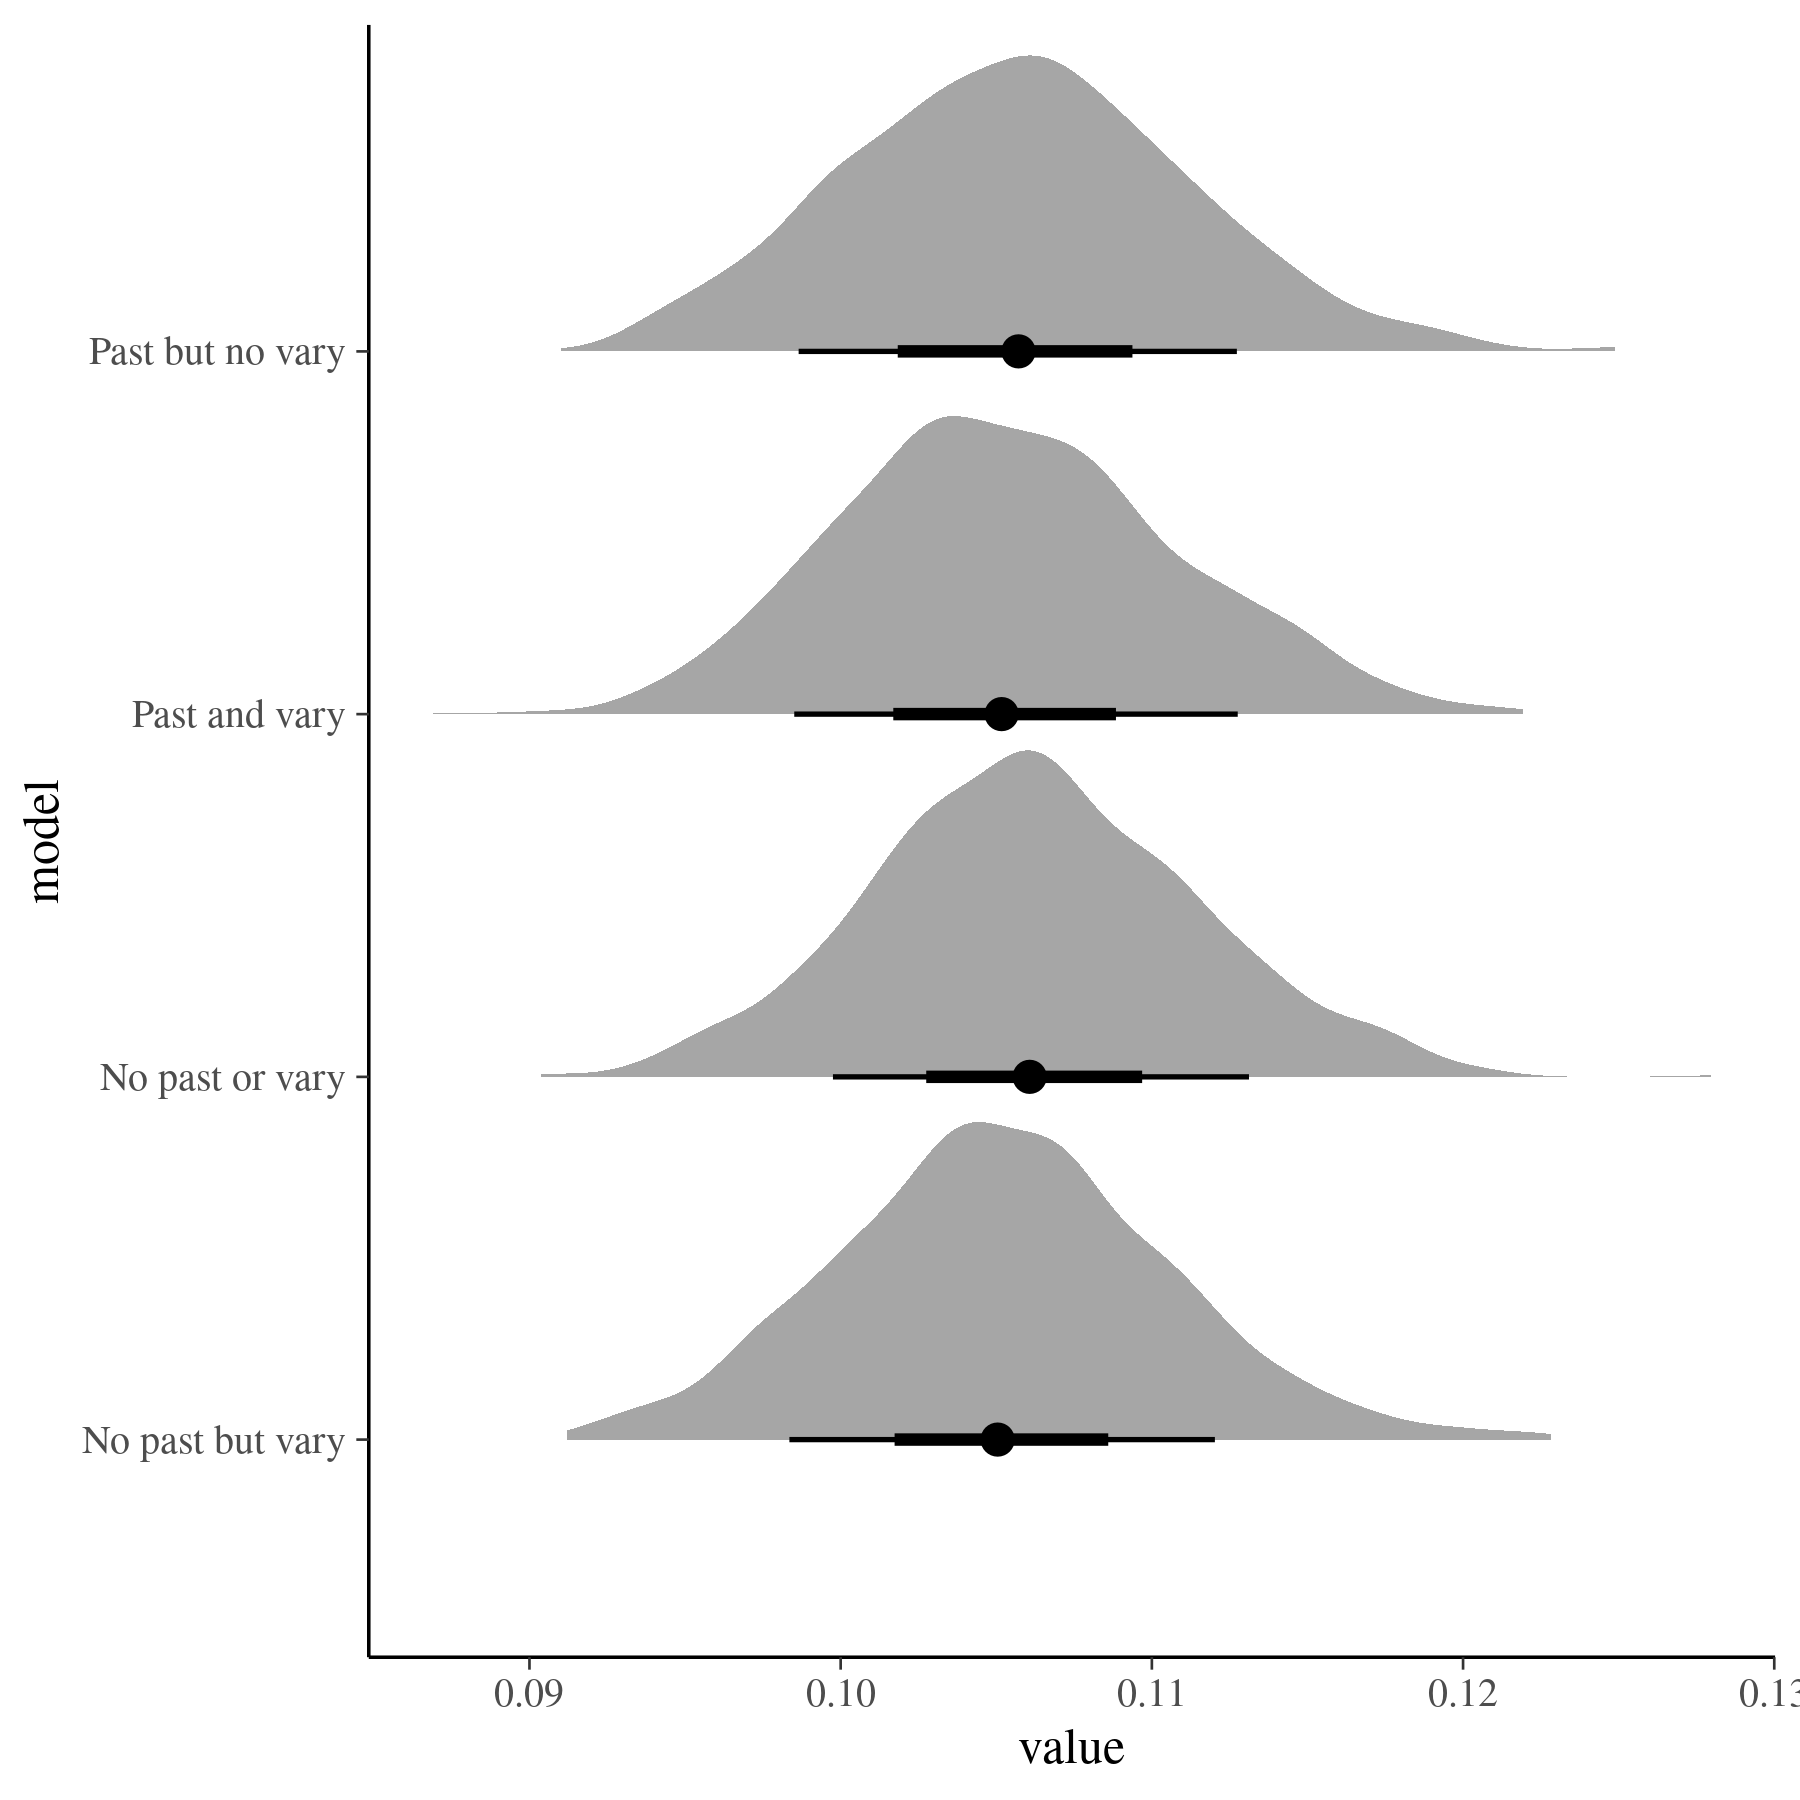
\includegraphics[width=\textwidth,height=0.5\textheight,keepaspectratio=true]{figure/cut_plot}
  \caption{Posterior estimates of the optimal cutpoints for each of the three models. The optimal cutpoint corresponds to the point which maximizes the true and false positive rates; this new cutpoint is used instead of 0.5 when estimating if an observation is the last observation of that species (i.e. goes extinct).}
  \label{fig:cut_point}
\end{figure}

Comparison of the in-sample AUC estimates between the four models reveals similar results as the selection criteria (Fig. \ref{fig:roc_hist}). While the parameter rich ``past and vary'' model has the greatest mean AUC when compared to the other three models, the other three models are quite similar. We chose to base our conclusions on the parameter rich ``past and vary'' model but these comparisons of model selection and adequacy illustrate the very small gain in performance that is achieved by allowing parameter effects to vary through time and including the historical covariates, though it appears that each of these choices on their own yield approximately equivalent models.
% ROC model comparison
\begin{figure}[ht]
  \centering
  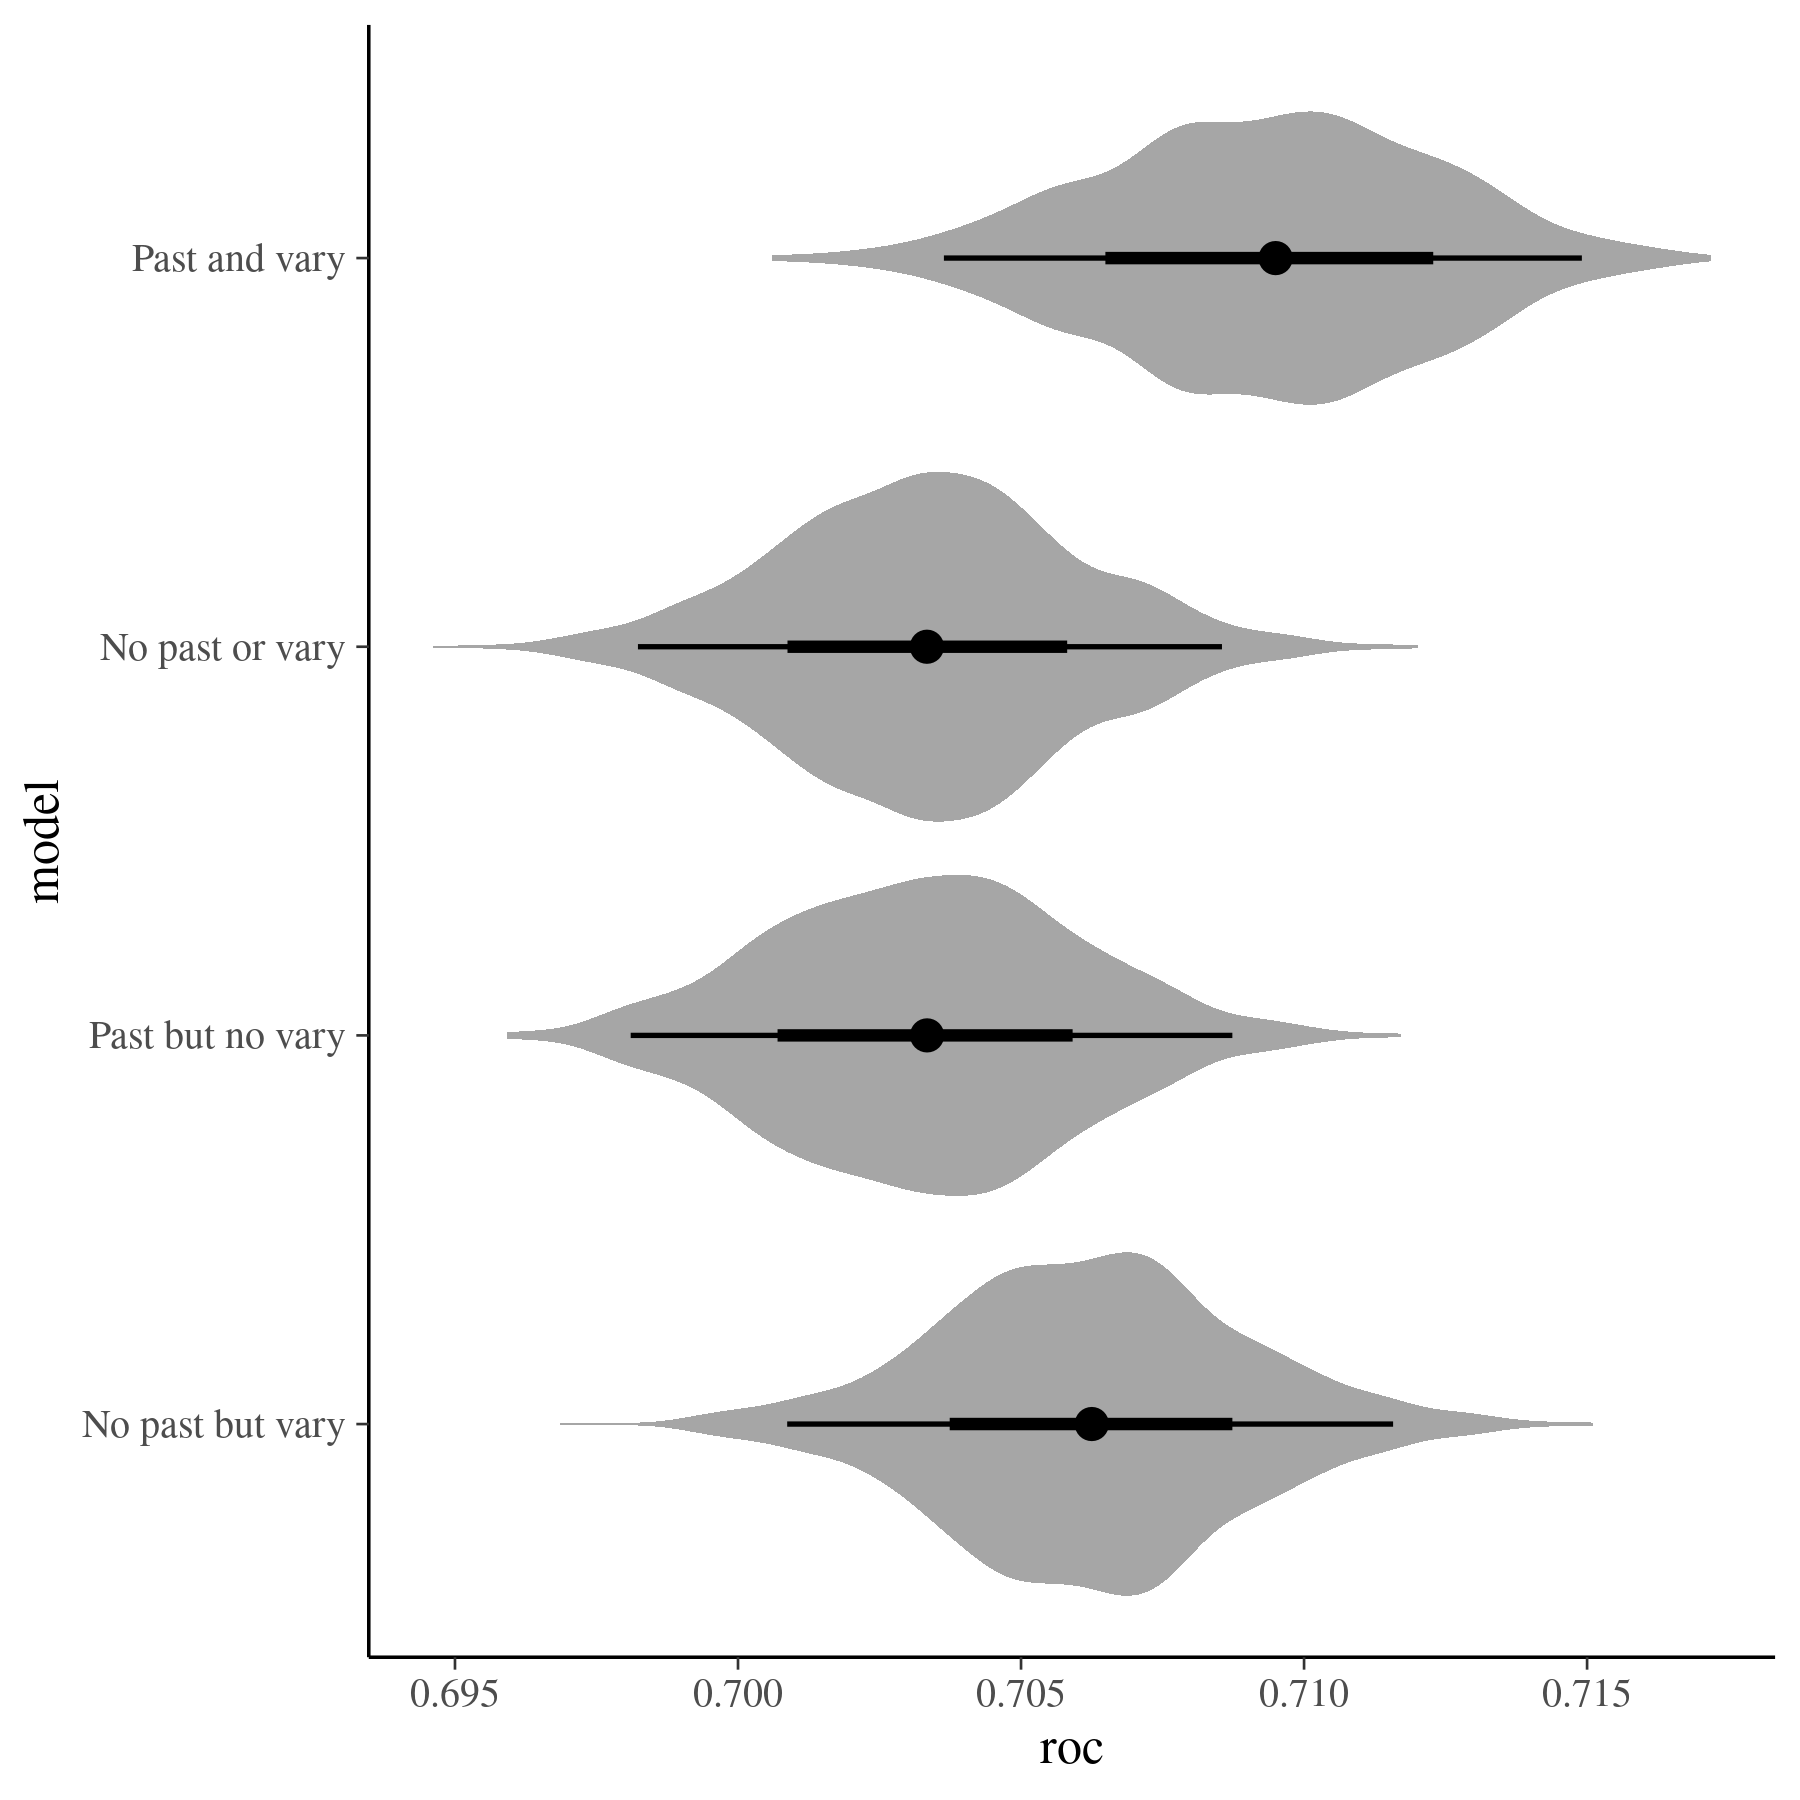
\includegraphics[width=\textwidth,height=0.5\textheight,keepaspectratio=true]{figure/roc_hist}
  \caption{Posterior predictive AUC estimates for each of the four models being compared. These estimates are calculated from each of the models posterior predictive distribution compared to the empirical values. Models with a higher AUC values indicate better performance over models with lower AUC values. AUC is bounded between 0.5 and 1.}
  \label{fig:roc_hist}
\end{figure}

Additional comparison of in-sample model performance at each of the time intervals reveals just how similar our four models are to each other (Fig. \ref{fig:roc_ts}). There are few if any obvious differences between the models in their performances.
% ROC model comparison time series
\begin{figure}[ht]
  \centering
  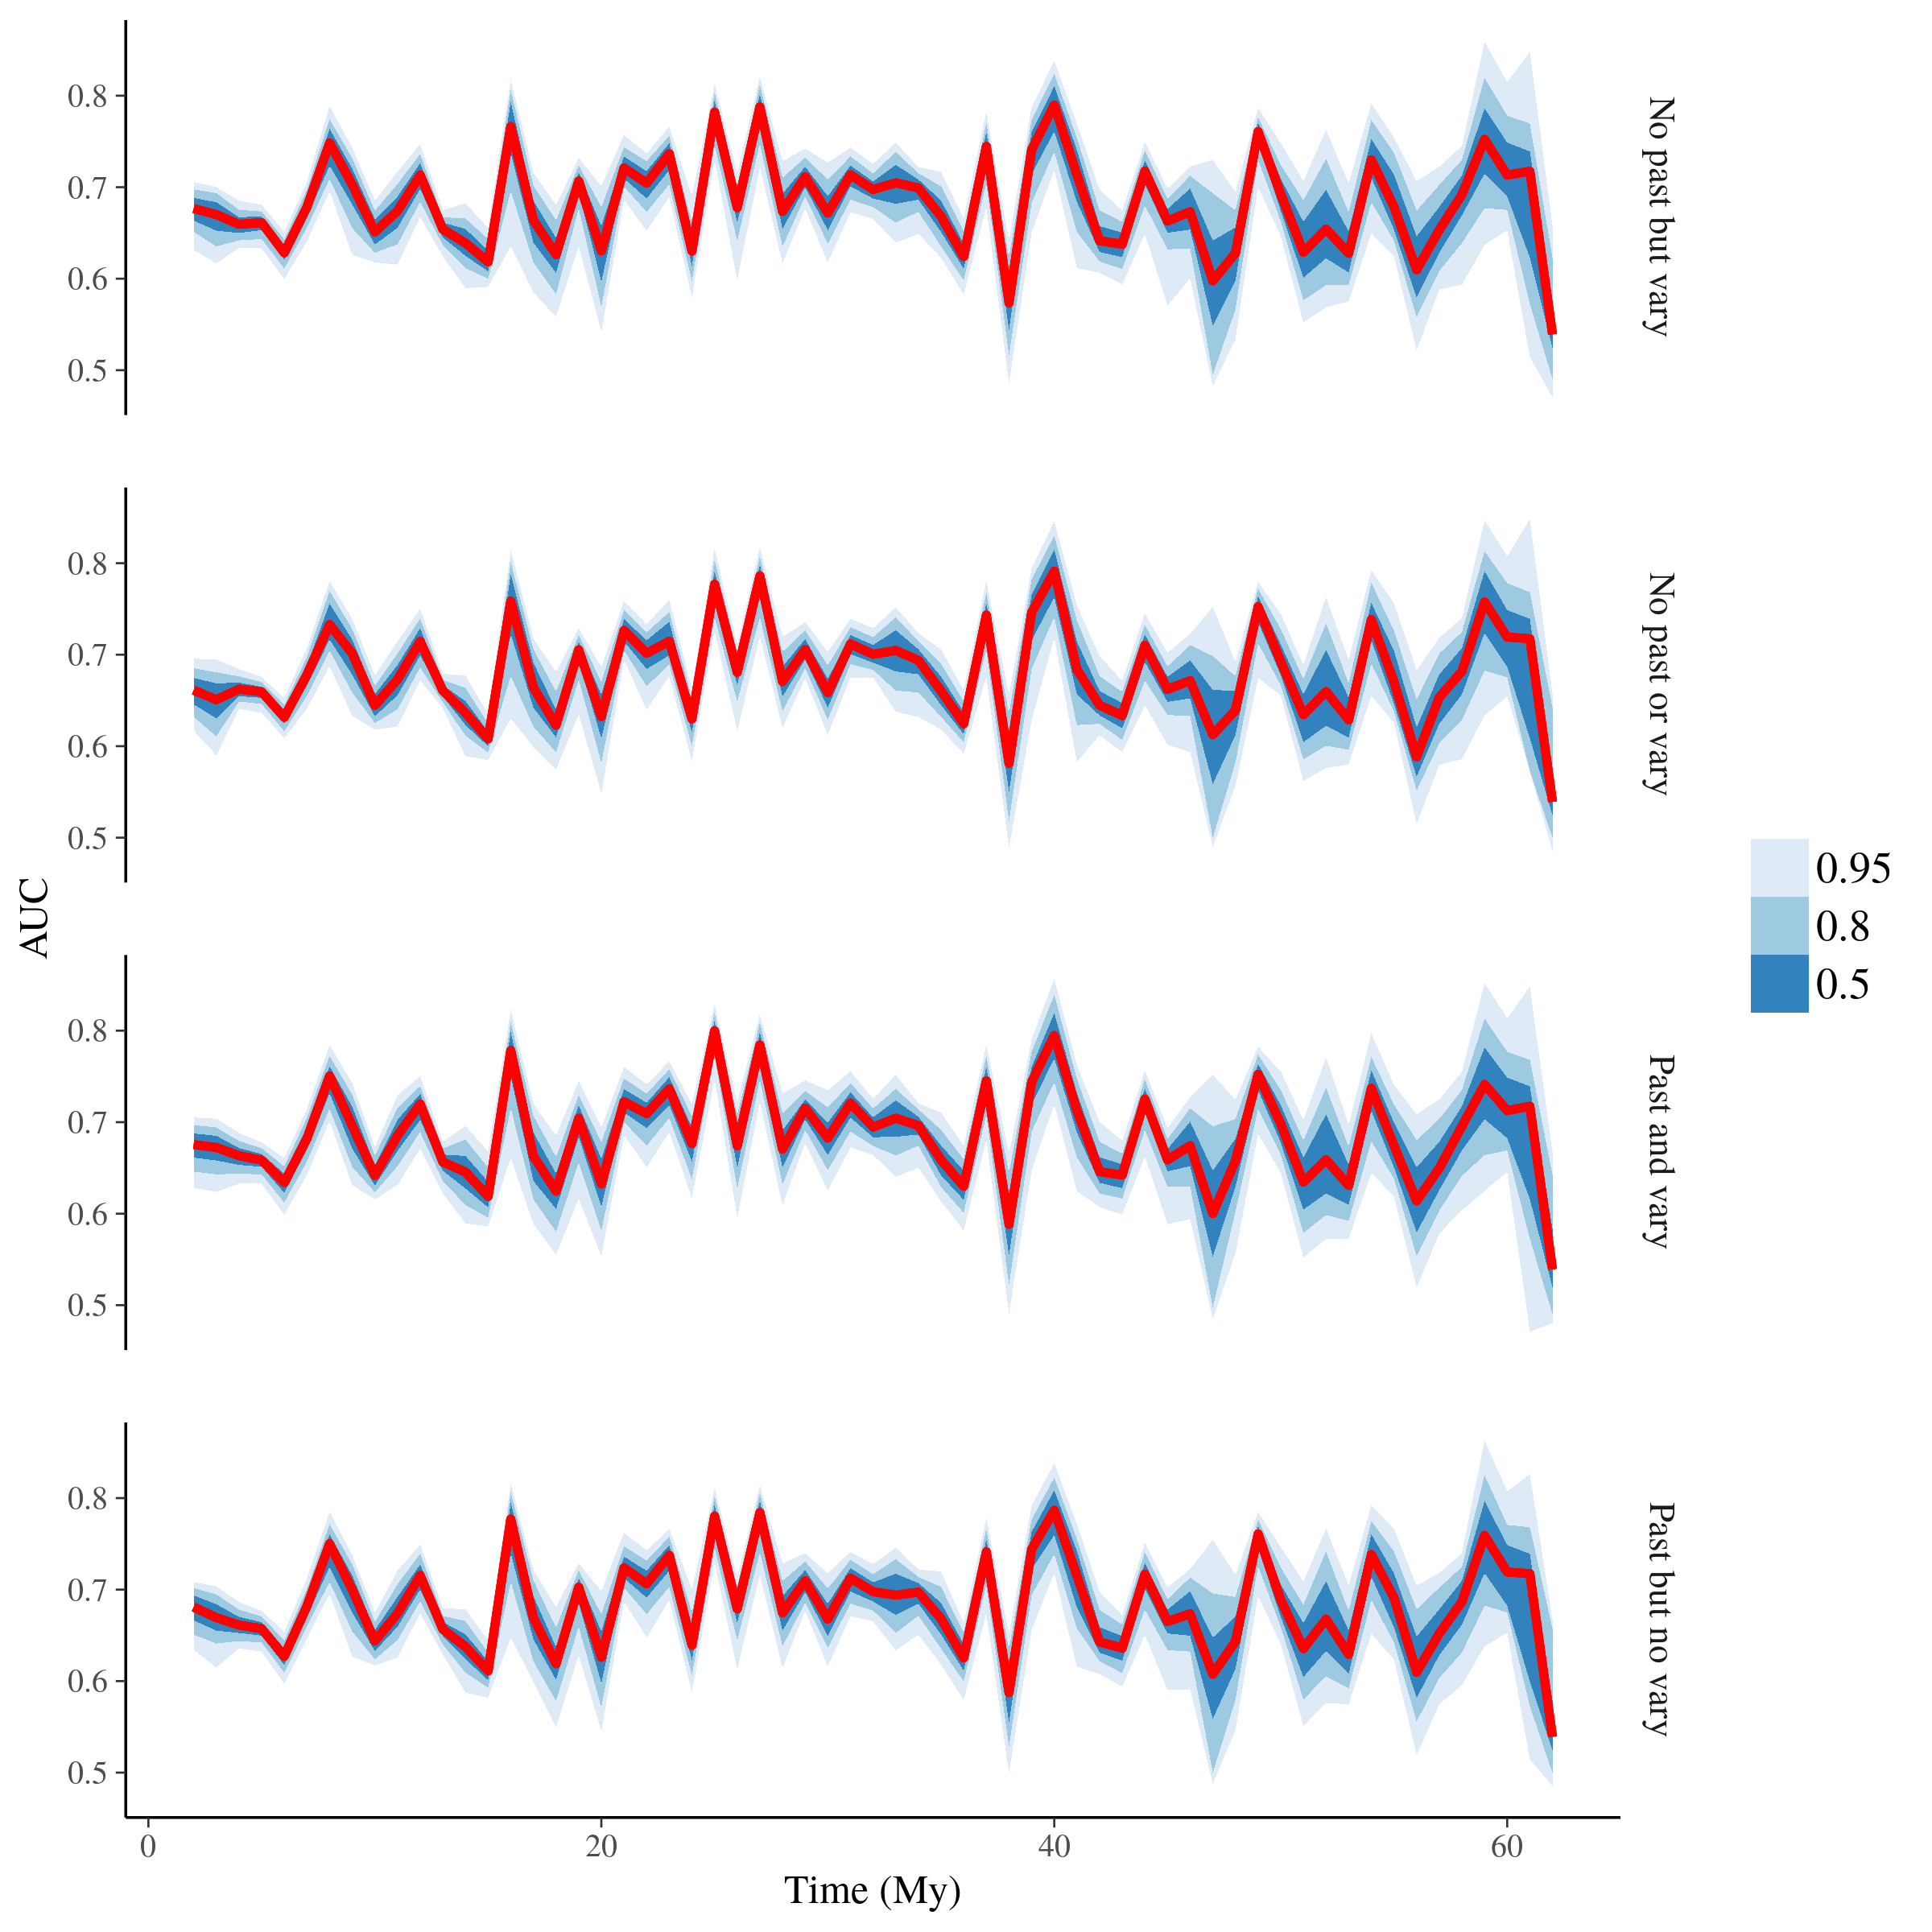
\includegraphics[width=\textwidth,height=0.5\textheight,keepaspectratio=true]{figure/roc_ts}
  \caption{Comparison between the posterior predictive AUC estimates for each of the time intervals for each of the four models. These estimates are reflections of each model's ability to fit the various time intervals. The red line corresponds to the median AUC value, while the envelopes correspond to multiple credible intervals. In all cases, higher values AUC indicate greater performance versus lower AUC values.}
  \label{fig:roc_ts}
\end{figure}

Because of the parameter rich ``past and vary'' model displays some modest improvements over the other models we choose this model for all further analysis.

\section{Cross-validation}

The approximate out-of-sample predictive performance for our selected model, as measured by AUC, is approximately identical to our in-sample performance (Fig. \ref{fig:fold_auc}). The quality of performance, however, is not great, with average out-of-sample AUC estimated to be just above 0.7 which is far from perfect. This result means that while we expect our model to yield consistent results when provided with new data, we do not expect that our predictions will be very accurate.
% ROC OOS estimate
\begin{figure}[ht]
  \centering
  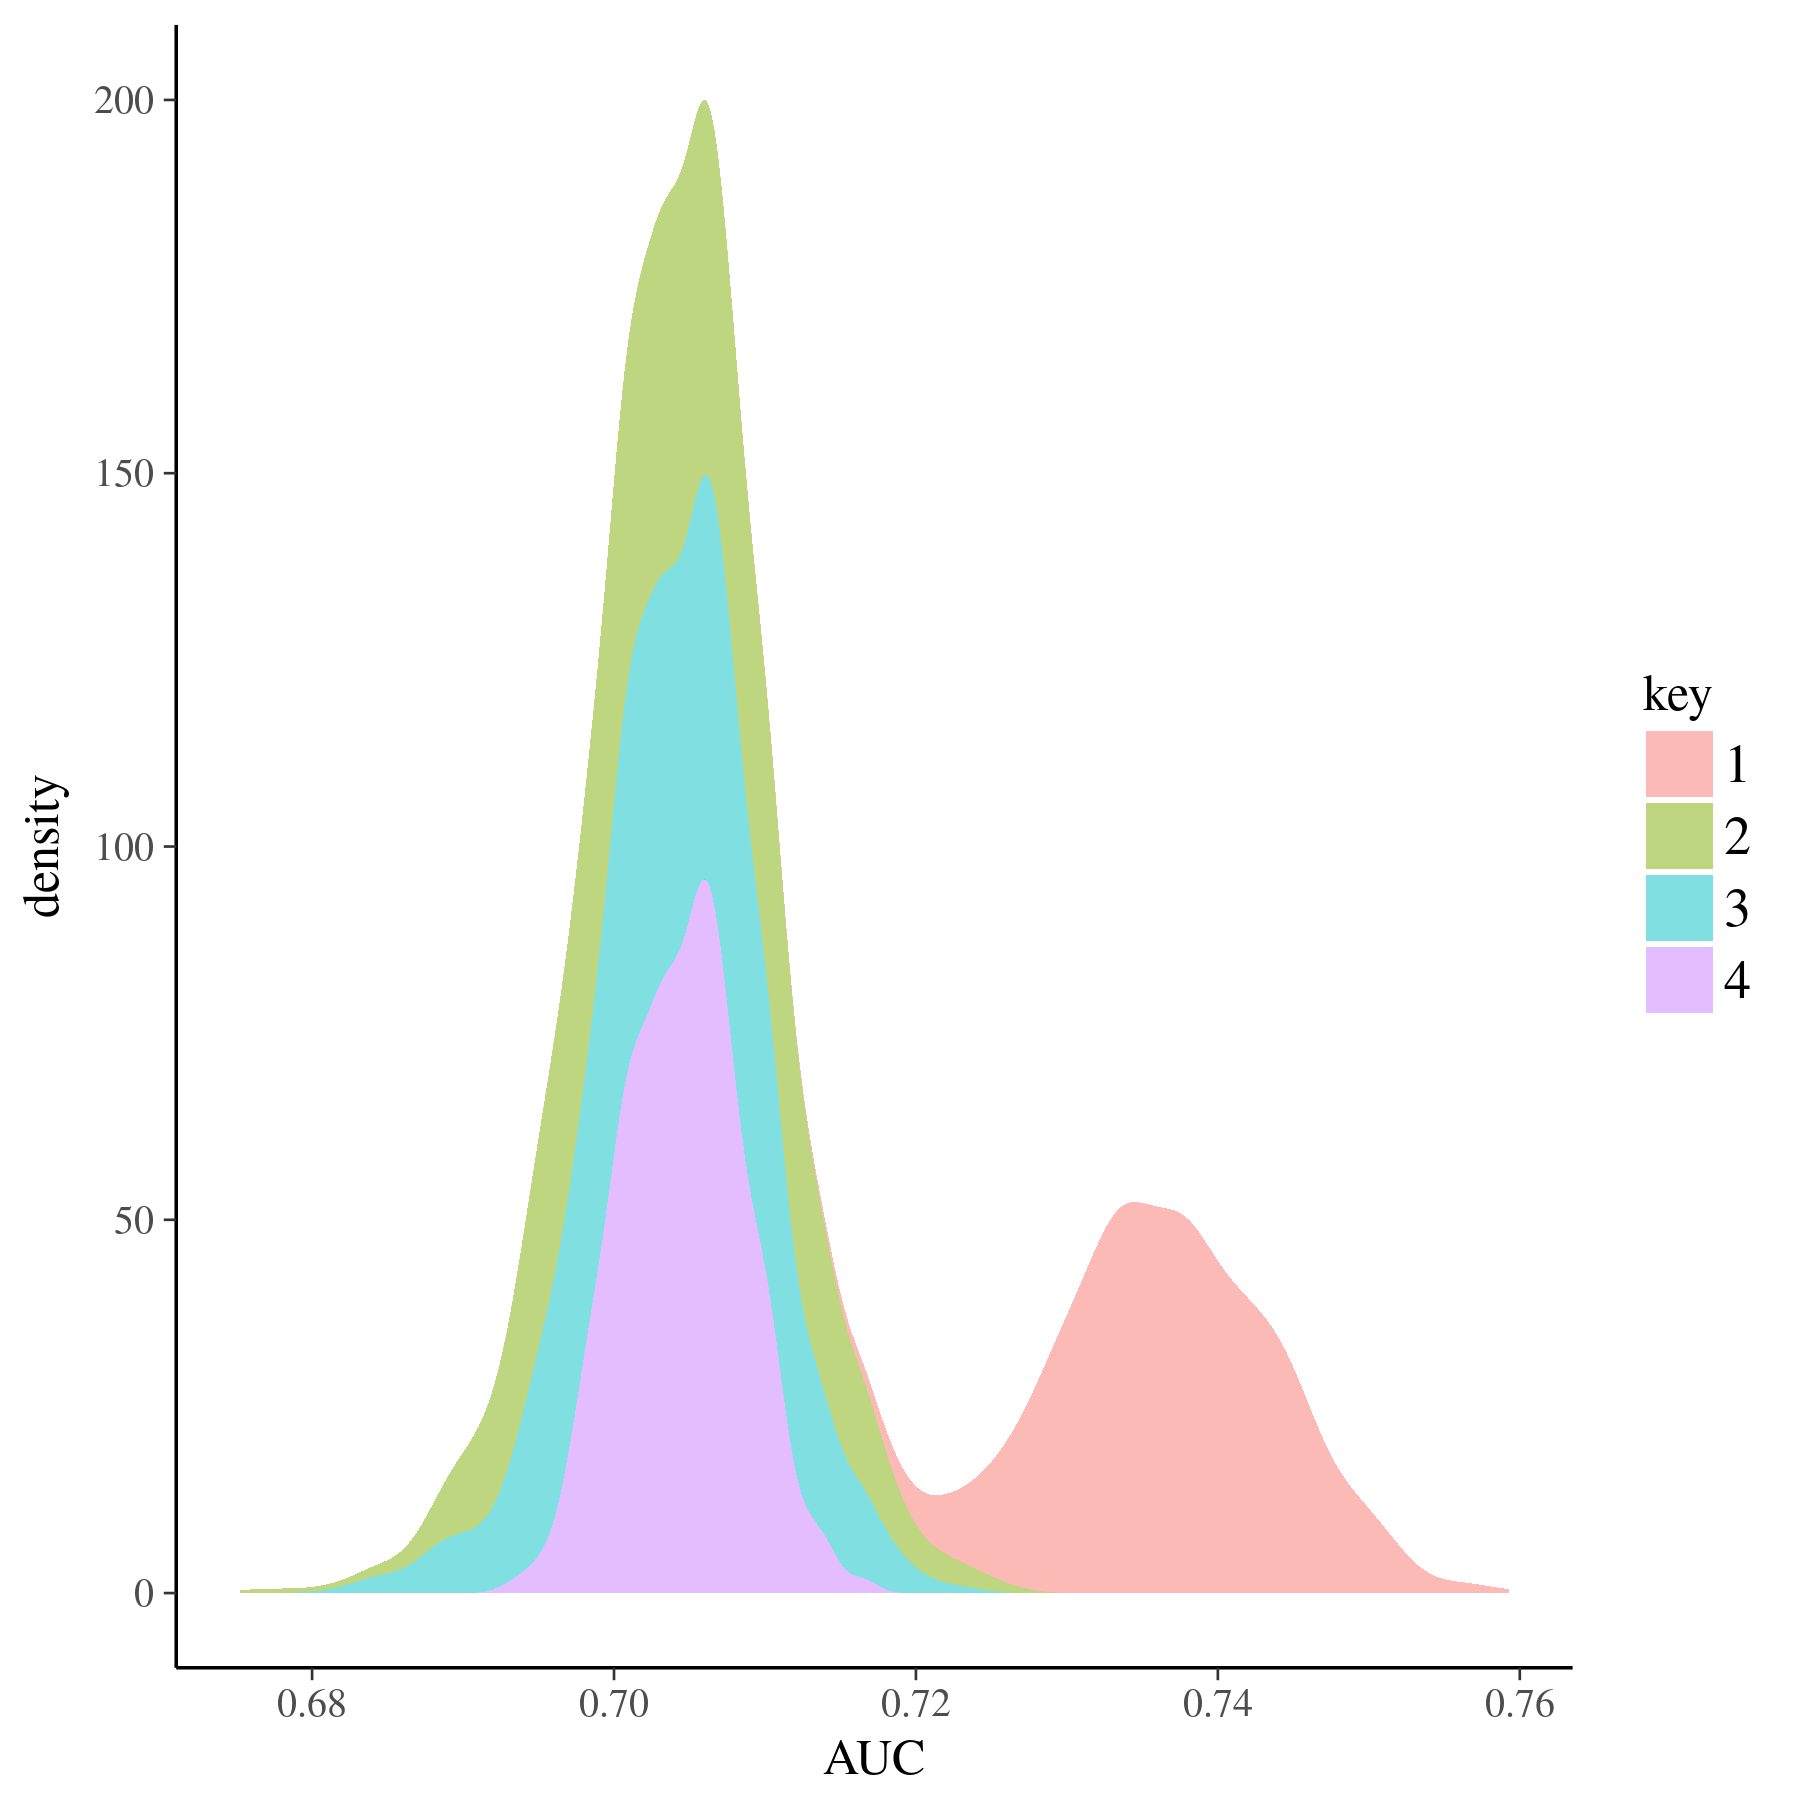
\includegraphics[width=\textwidth,height=0.5\textheight,keepaspectratio=true]{figure/fold_auc}
  \caption{Results from our five-fold cross-validation of the time-series. Each labeled distribution of AUC values correspond to expected out-of-sample performance as estimated from that fold. Each fold represents a section of data being predicted from a model fit to all data before the start of that fold. Given that there are only five folds, performance is measured from model predictions to 4 of the folds. Folds are labeled from oldest to youngest, with the oldest fold only being predicted by a single previous fold and the youngest fold being predicted by the four previous folds.}
  \label{fig:fold_auc}
\end{figure}

%When our cross-validation estimates are presented for each time interval, 
%% ROC OOS estimate time series
%\begin{figure}[ht]
%  \centering
%  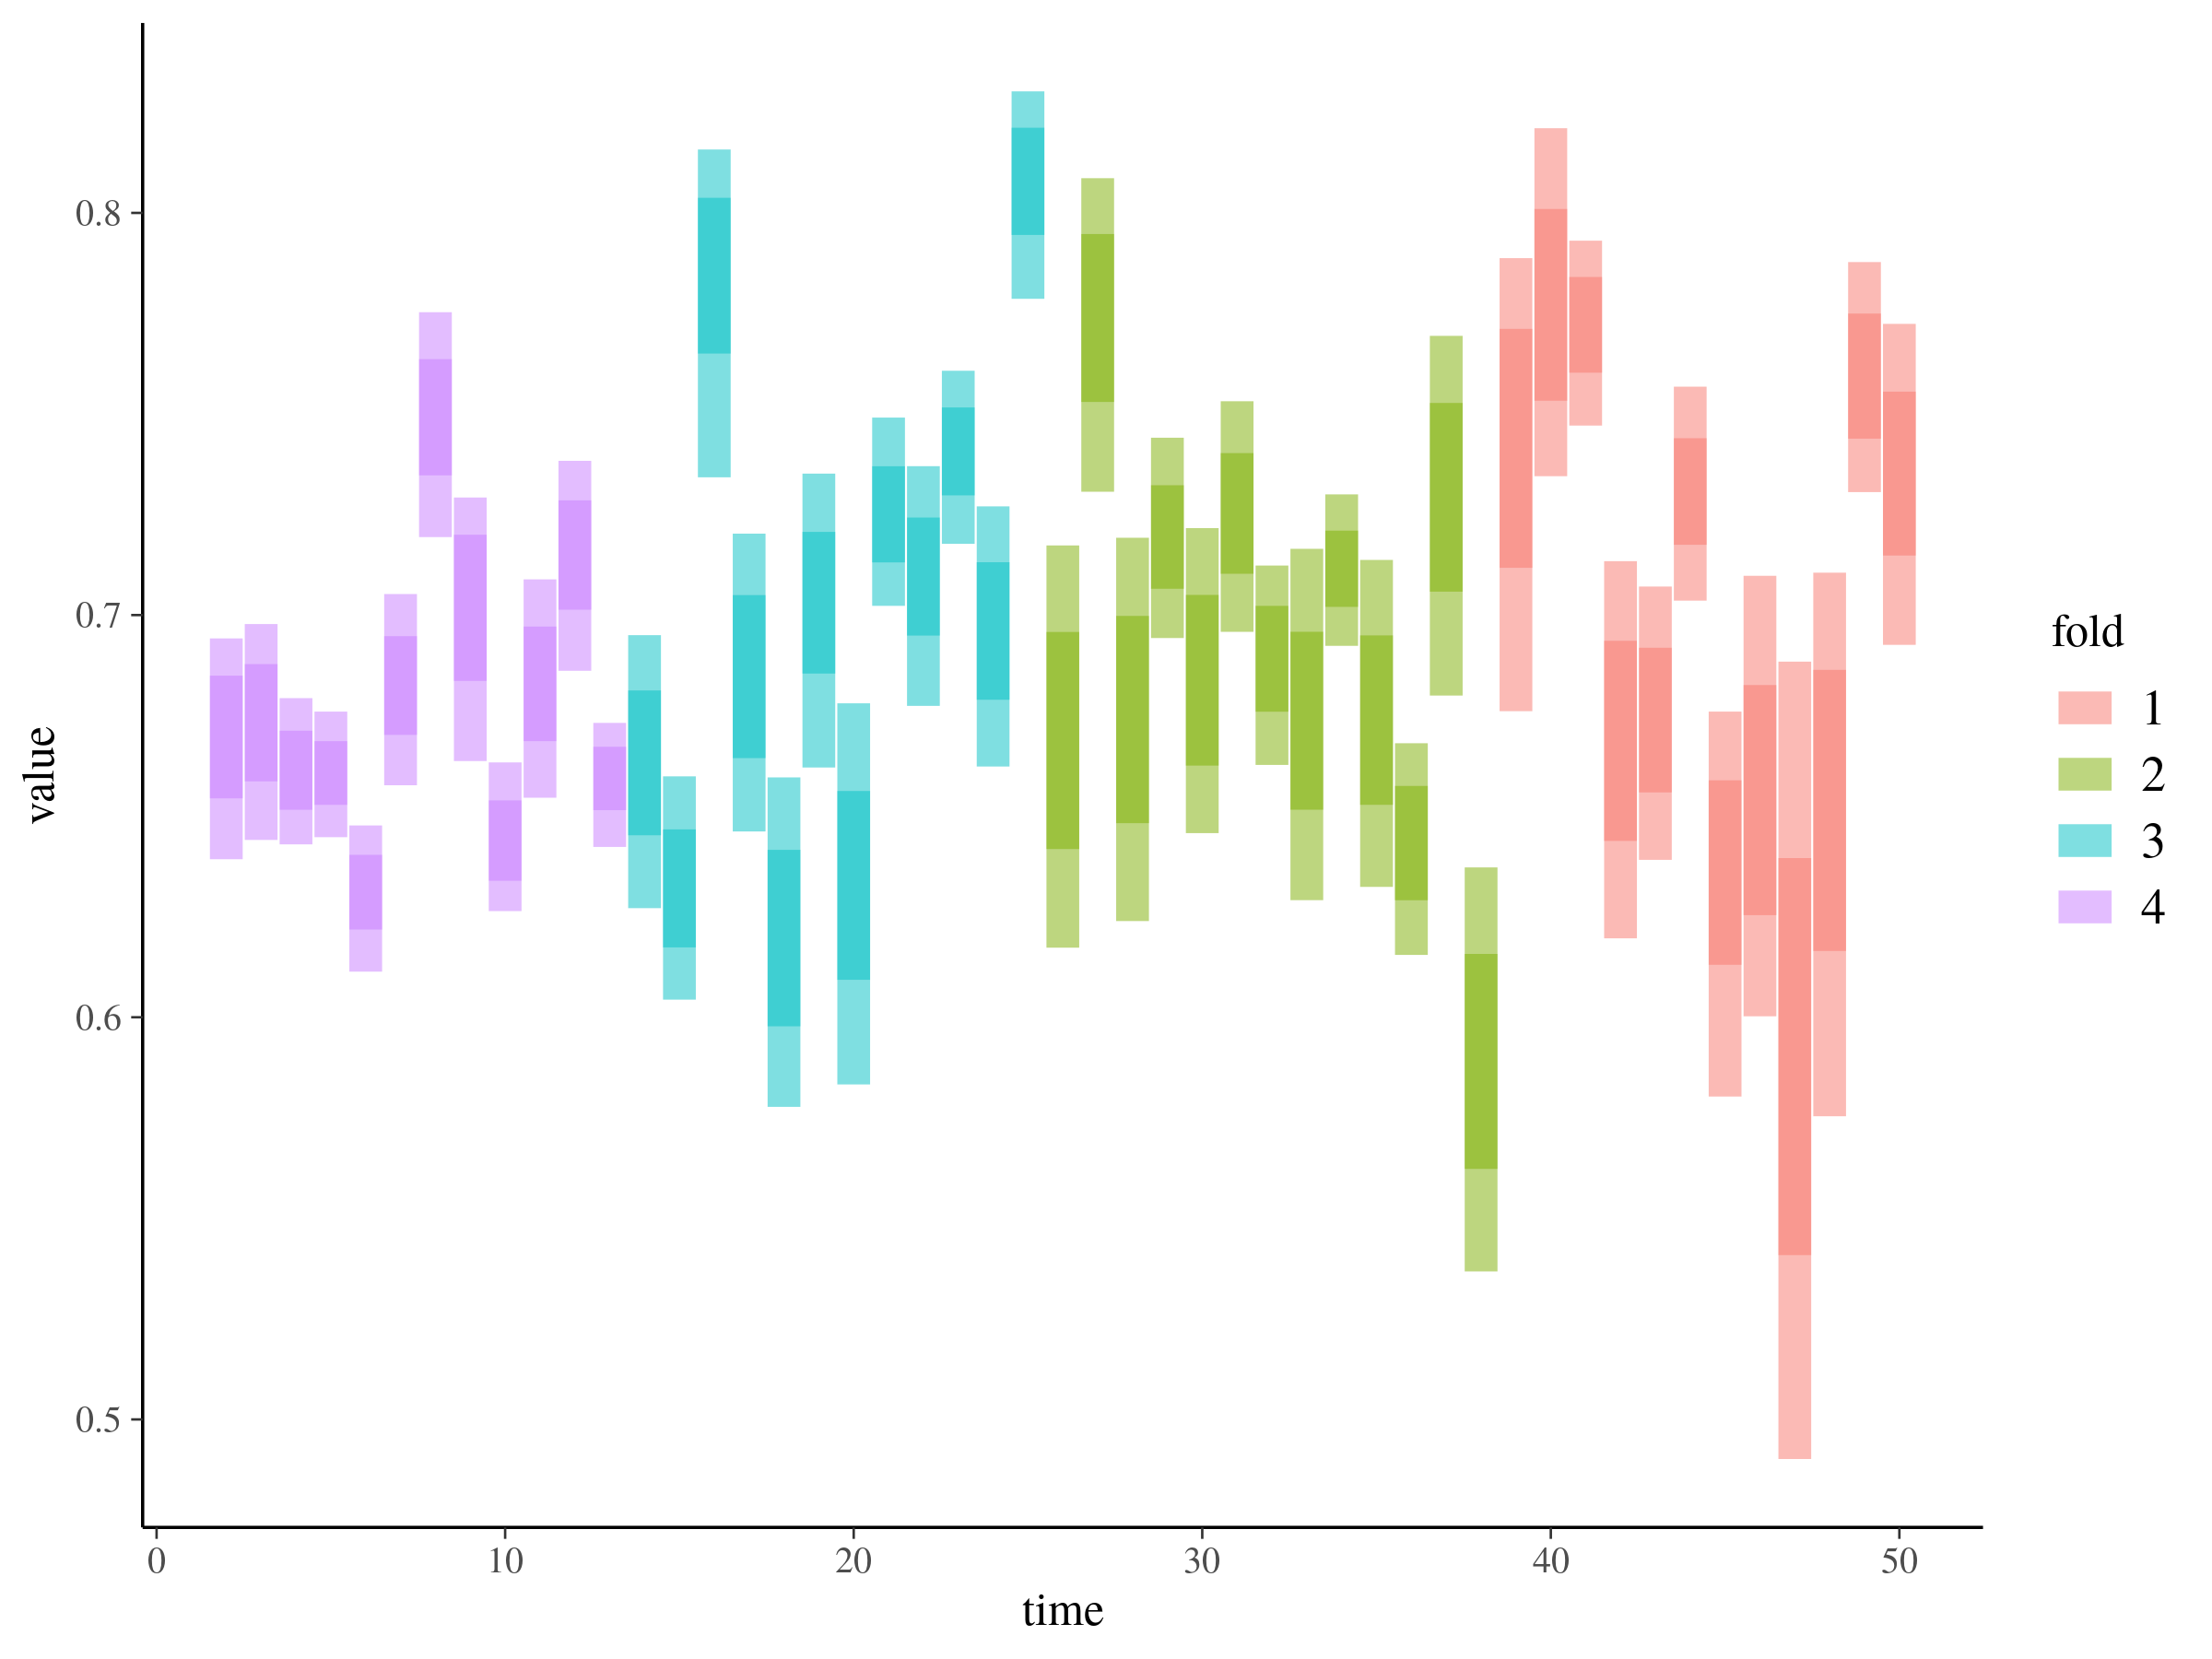
\includegraphics[width=\textwidth,height=0.5\textheight,keepaspectratio=true]{figure/fold_auc_time}
%  \caption{Approximate out-of-sample AUC values calculated for each of the My intervals using five-fold cross-validation of the time series. The AUC of the individual My intervals within each fold is plotted to highlight the heterogentity in performance within and between folds. The AUC estimates from each fold are labeled and are numbered from oldest to youngest.}
%  \label{fig:fold_auc_time}
%\end{figure}


\section{Parameter estimates}

The overall average probability of a species going extinct during any interval is very low (Fig. \ref{fig:effect_est}). This result means that even if covariate effects are very large on the log-odds scale, when compared on the probability scale will only produce a minor change in probability of extinction. This is one of the hardest parts of logistic regression for people to understand. Effect sizes are on the log-odds scale but prediction is on the probability scale. When the intercept term is very negative or positive (greater than 2), covariate effects are fighting over an increasingly small amount of probability. Logistic regressions are easiest to interpret when the intercept term is approximately 0; this is a fundamental difficulty of dealing with very uneven data sets.

As expected, a species with greater than average geographic range is expected to have a greater probability of surviving than a species with average or less than average geographic range (Fig. \ref{fig:effect_est})

We estimated an overall positive effect of the change in geographic range on extinction probability; this means that a species gaining in geographic range between that observation and their previous observed geographic range is associated with a greater extinction risk than a species which decreased in geographic range (Fig. \ref{fig:effect_est}). This sign of this result is consistent with virtually all previous analyses of the relation between geographic range and extinction.

We estimated an overall positive effect of both global temperature and the lag of global temperature with species extinction probability (Fig. \ref{fig:effect_est}. This type of effect means that when global temperature is above the Cenozoic average, we would expect higher than average extinction risk. Similarly, if global temperature was above the Cenozoic average in the time interval before the current one, we would also expect higher than average extinction risk. This means that during a run of above Cenozoic average global temperatures (2+ intervals) we would expect an even greater extinction risk than if just the current interval is of above average temperature. These results imply that, on average, the species during Paleogene had a greater extinction probability that species during the Neogene.

% effects, average
\begin{figure}[ht]
  \centering
  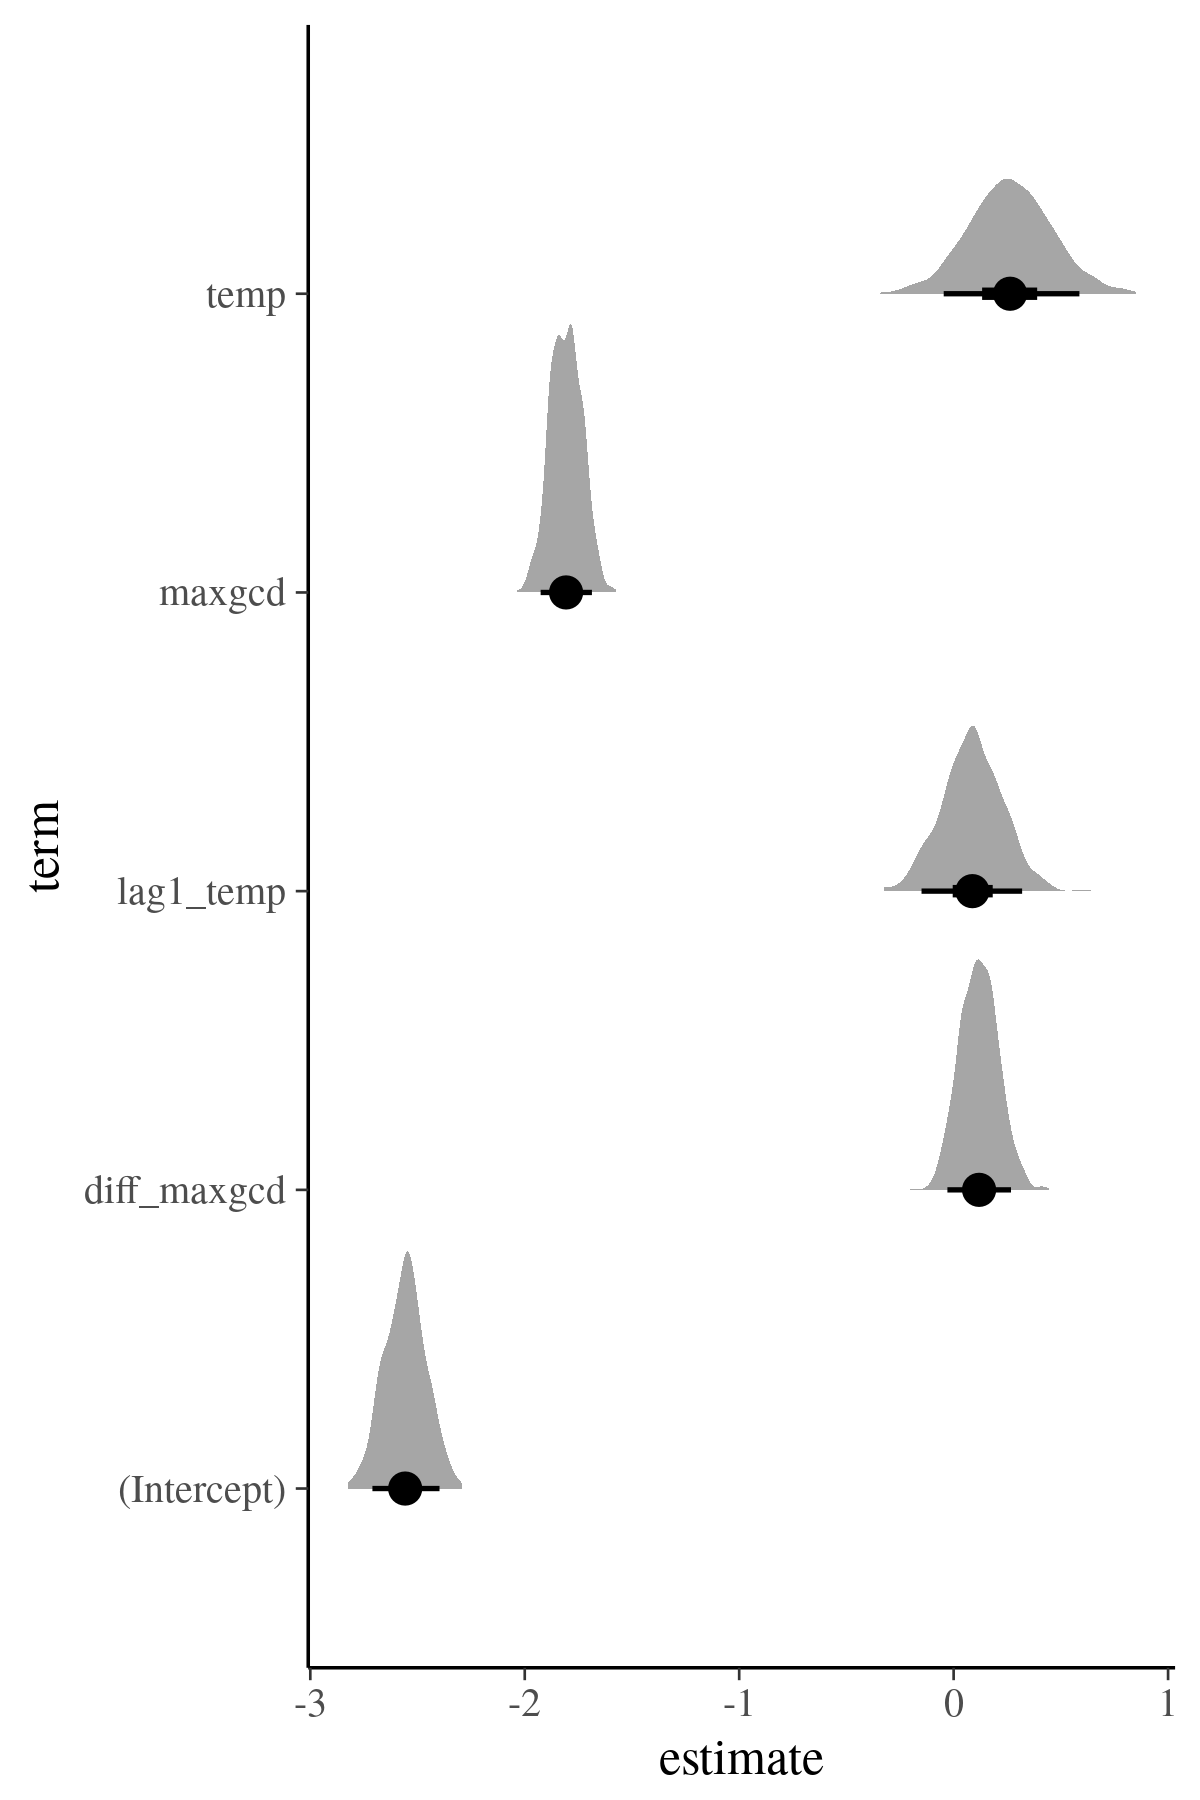
\includegraphics[width=\textwidth,height=0.5\textheight,keepaspectratio=true]{figure/effect_est}
  \caption{Posterior estimates for the top-level covariate effects. These effect estimates are effectively the weighted average of the estimates for each of the time intervals, for each of the phyla analyzed. Presented are posterior densities with the median estimate labeled along 80\% credible intervals at the bottom of the density.}
  \label{fig:effect_est}
\end{figure}


The overall effect averages described above do not reflect the between time-interval variance of the effects. While the effect of geographic range has a consistent sign for the entire Cenozoic, the effects of the other covariates do not have a consistent sign (Fig. \ref{fig:effect_time_group}). 

% effects, time series
\begin{figure}[ht]
  \centering
  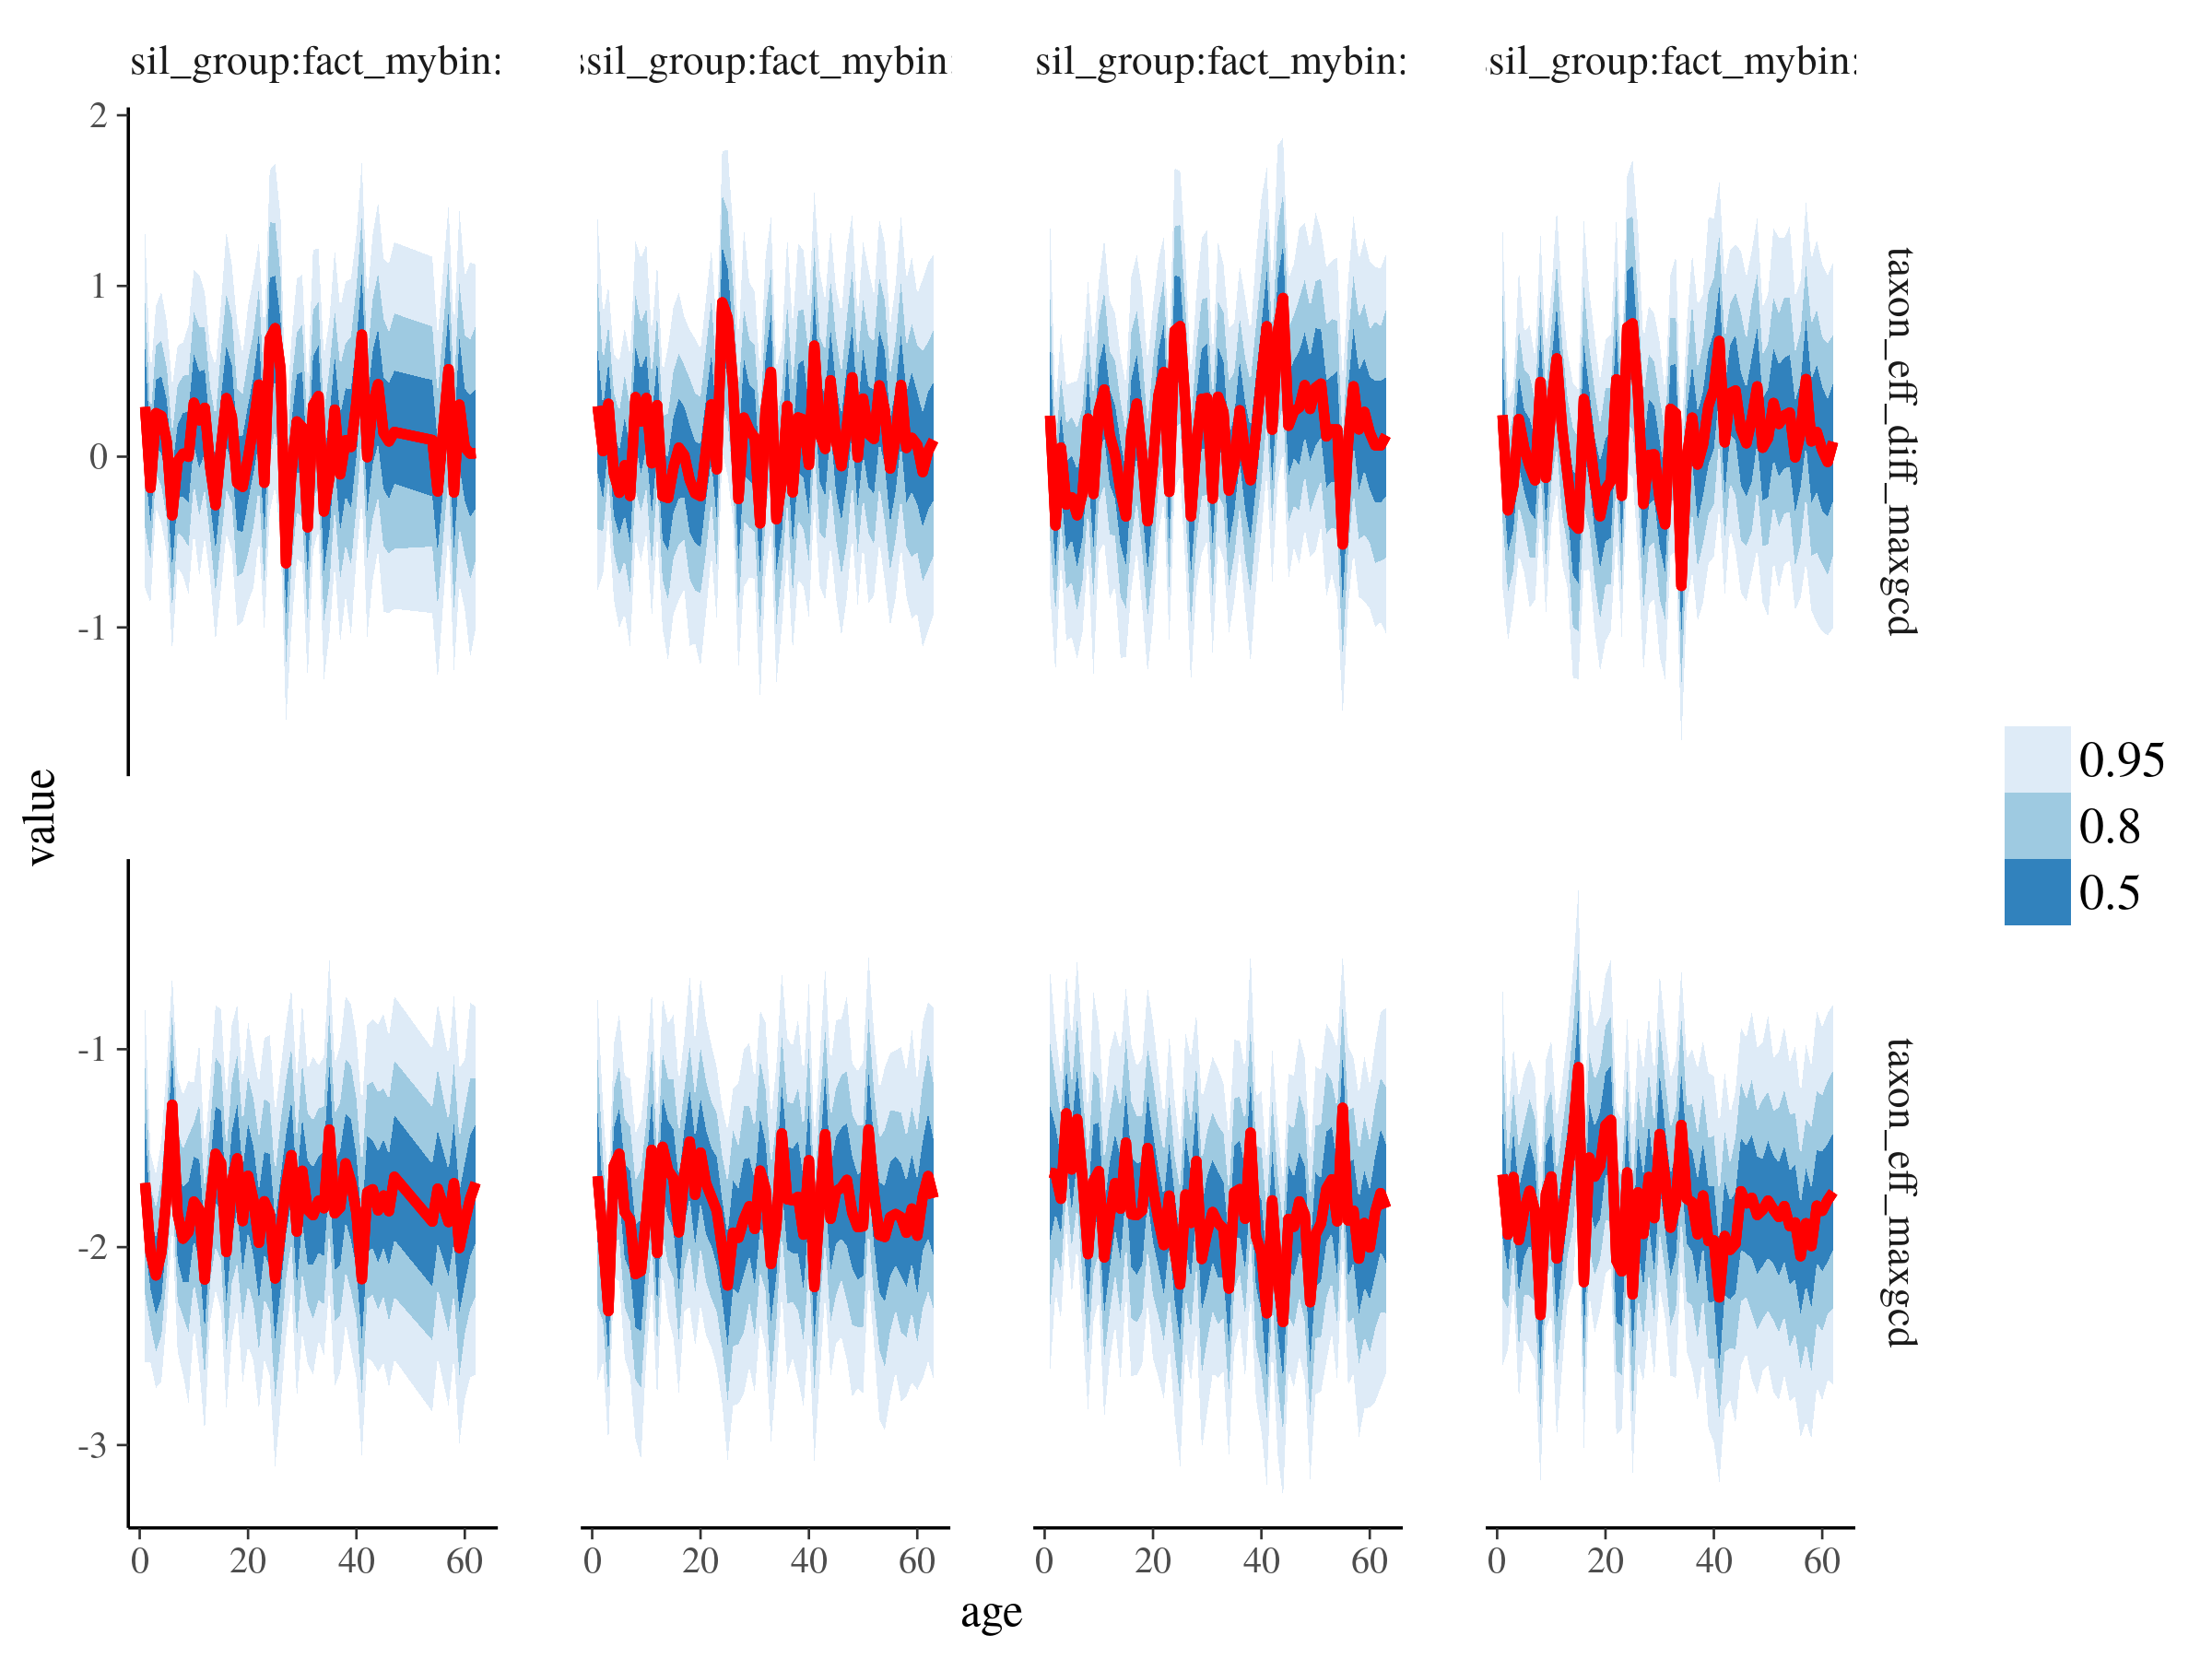
\includegraphics[width=\textwidth,height=0.5\textheight,keepaspectratio=true]{figure/eff_time_group}
  \caption{Effects of the four covariates as estimated for all time intervals and for each phyla. For each time series, the red line corresponds to the median estimate for each interval, while the envelopes represent various credible intervals as labeled.}
  \label{fig:effect_time_group}
\end{figure}


% effect of age at observation

% average hazard
The hazard function describes how age of observation impacts probability of extinction. Hazard is estimated for each phylum for the range of ages observed within the phylum. The matrix \(A\) describes the effect of age on extinction probability for age at observation (rows) by phylum (columns). The phylum-level averages of the effect of age of observation on extinction \(\delta\) are themselves drawn from a distribution centered around 0.


Figure \ref{fig:hazard_baseline} is a graph of the average hazard associated with age of observation. This graph illustrates how average extinction risk increases with age for the first few million years before leveling off. A species reaches highest age-related probability of extinction at 10 million years, after which the median becomes volatile until a duration over 30 million years. The flat-ness of the median estimate and the homogeneity of variance durations between approximately 30 million years to under 60 million years is due to the lack of species having survived over 30 million years, which inherently means that these estimates are based on less information and are shrunk towards the overall average while reflecting more and more of our prior uncertainty over time. 

\begin{figure}[ht]
  \centering
  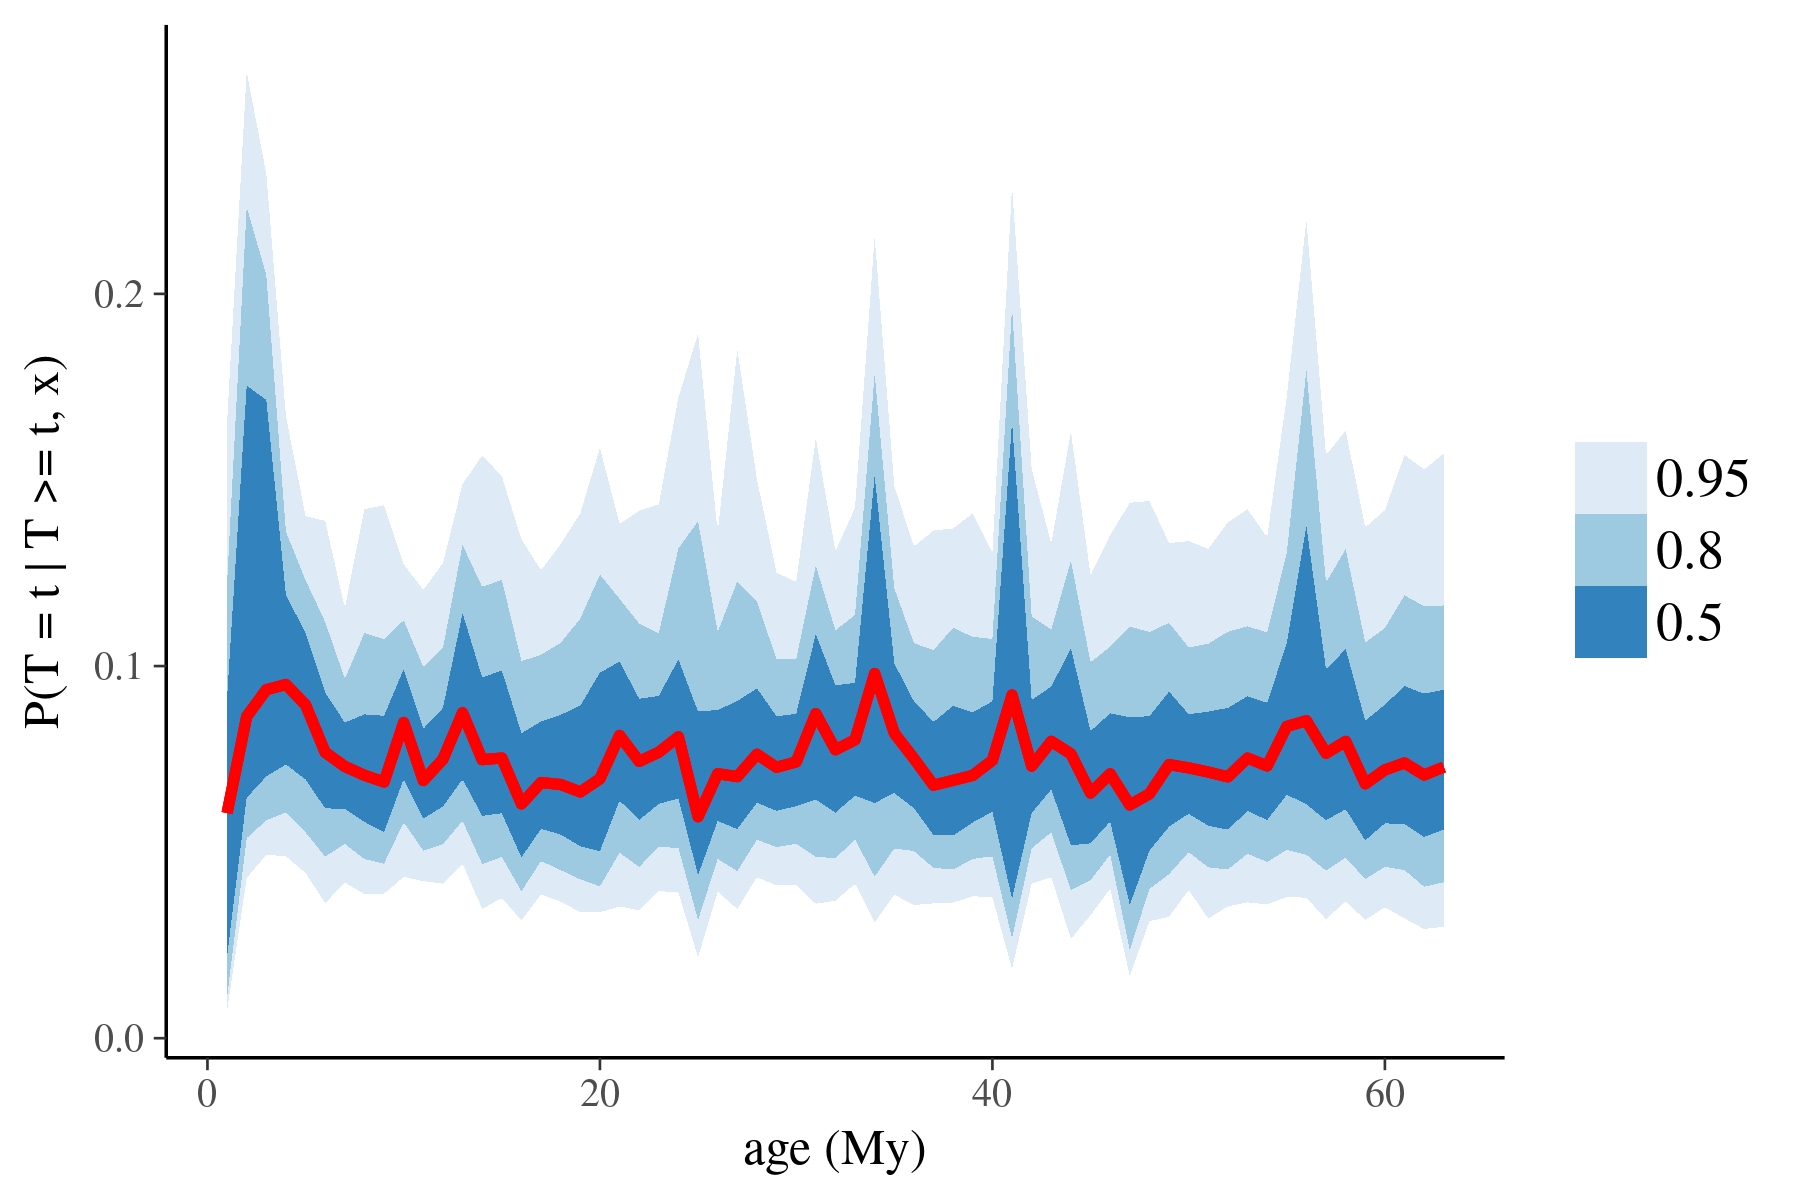
\includegraphics[width=\textwidth,height=0.5\textheight,keepaspectratio=true]{figure/hazard_baseline}
  \caption{Average hazard estimates based on all all observed species ages in millions of years. Hazard in discrete-survival analysis is the probability of going extinct at a given age having survived up to that age. Overall hazard was calculated using the phylum average intercept and assuming all covariates equaled 0. The red line is the median hazard estimate along with 50\%, 80\%, and 95\% credible intervals.}
  \label{fig:hazard_baseline}
\end{figure}

The hazard associated with the individual phyla have broad similarities with the overall hazard estimates (Fig. \ref{fig:hazard_bygroup}). In all four cases, hazard increases over the first 10 million years of a species duration. However, the rate of increase in hazard varies between the phyla, with forams and radiolarians having the most pronounced increase with age. Radiolarians also have the lowest initial hazard of the phyla, followed by forams and calcareous nannoplankton. In contrast, diatoms have the highest initial hazard of the phyla while having the smallest change hazard with age. 

Optimal cutpoint between 0.1 and 0.11 percent. We estimate that the effect of age of observation on extinction can reach this threshold after XX My at YY\% posterior probability.

\begin{figure}[ht]
  \centering
  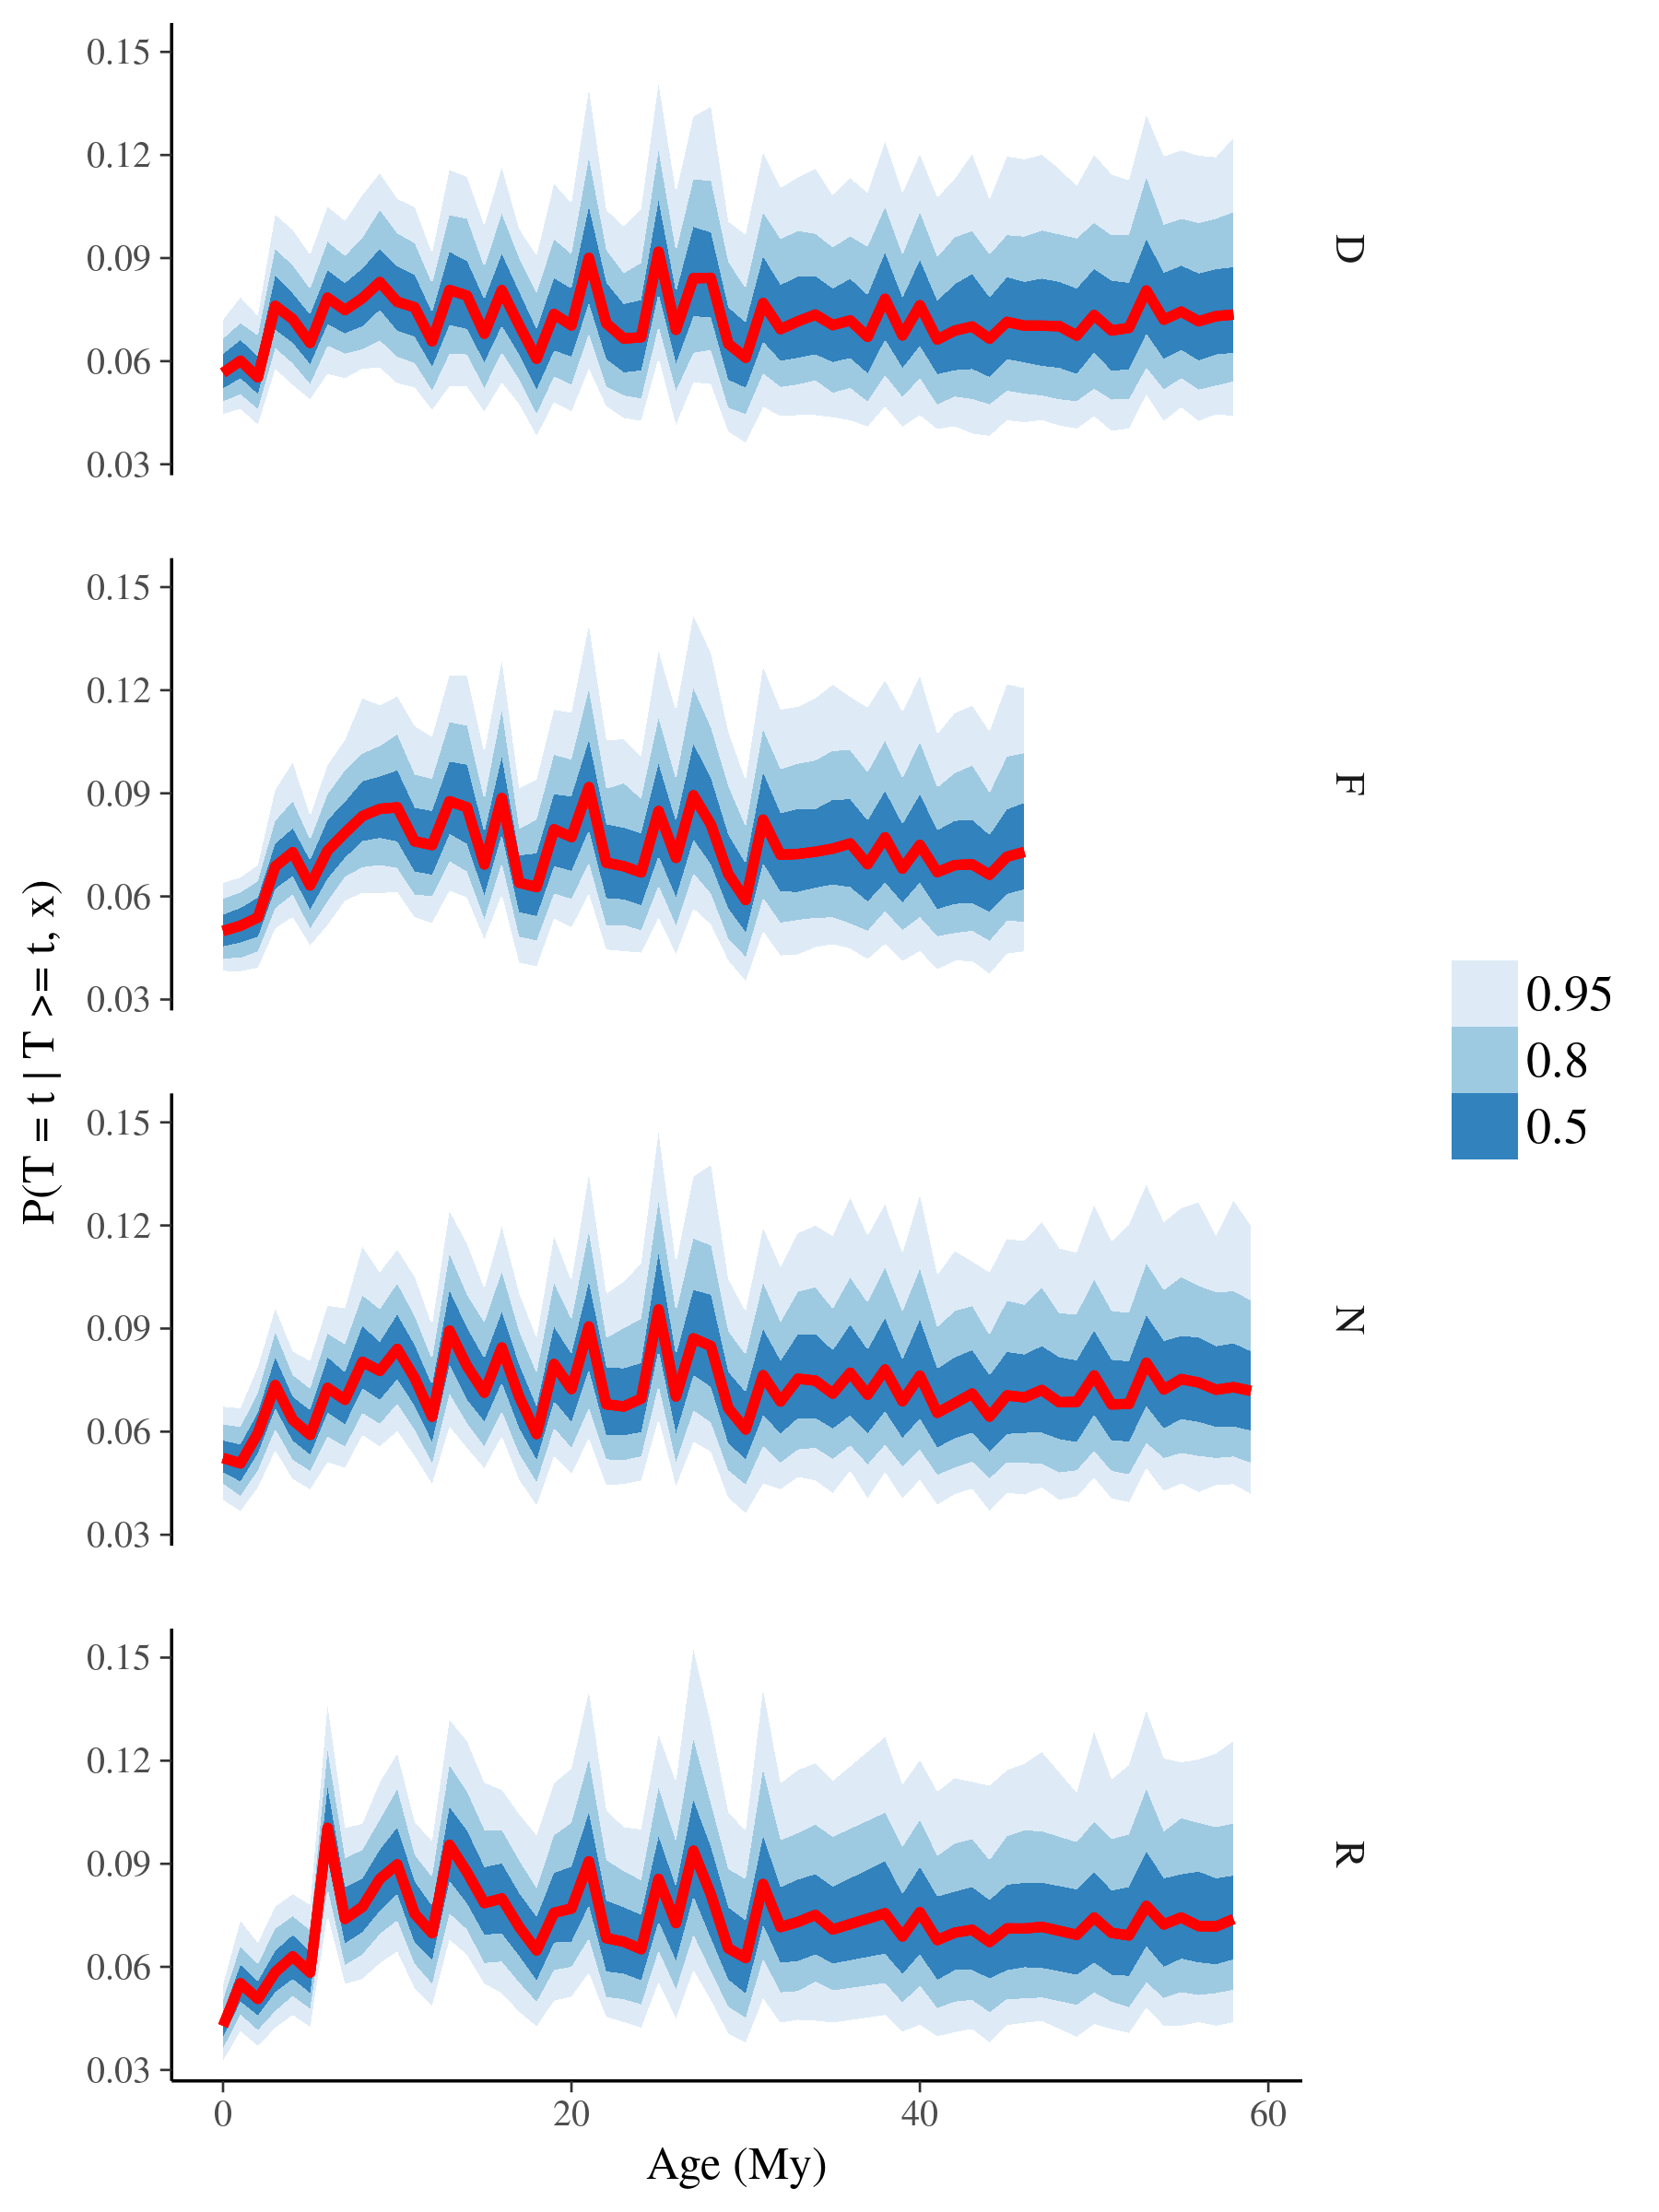
\includegraphics[width=\textwidth,height=0.5\textheight,keepaspectratio=true]{figure/hazard_bygroup}
  \caption{Hazard estimates for each of the phyla analyzed here. The red line is the median hazard estimate along with 50\%, 80\%, and 95\% credible intervals.}
  \label{fig:hazard_bygroup}
\end{figure}


% variance components
There are multiple levels and sources of variance in our model. Each of the grouping factors account for some amount of variance in the data. The first ``level'' of variance is the data level or the variance in the observed data (the model response). In the context of regular linear regression, this variance is equivalent to the residual variance. In the context of logistic regression, however, this value is not an inherent part of the model.

There are then two non-nested sources of the second ``level'' of variance: intercept and slopes varying by time of observation, and a mean-zero age at observation varying intercept. Each of the elements of the vector of scale terms \(\tau_{B}\) describe the within-phyla variance for the intercept and the slope terms for the covariates. Similarly, the scale term \(\sigma_{A}\) is a scalar that describes the within-phyla variance of the effect of age at observation. 

The final ``level'' of variance the phyla-level: the between phyla variance for the intercepts and regression coefficients \(\tau_{\alpha}\), and the between phyla variance for the effect of age at observation \(\sigma_{\delta}\). 

The greatest source of variance accounted for by the grouping factors is the between phylum variance in the model intercept (Fig. \ref{fig:variance_components}); this is the first element of \(\tau_{B}\). All of the other scale terms have approximately equal estimates, which means that they contribute a similar amount to the structure underlying the data. For example, the within-phyla effect of geographic range on extinction probability is associated with approximately as much variance as there is between the phyla themselves.

This result means that, given this model, the greatest contributor to differences in extinction risk over time is when a species is present. In comparison, the covariates we studied individually contribute only a limited amount to the variation in extinction. Similarly, while age at observation does contribute to some differences in extinction risk (Fig XXX age effect), this effect is most likely overwhelmed by the importance of when that observation takes place.

The variance in effects contributed by the phyla is approximately equal to the variance in those effects due to differences over time.


\begin{figure}[ht]
  \centering
  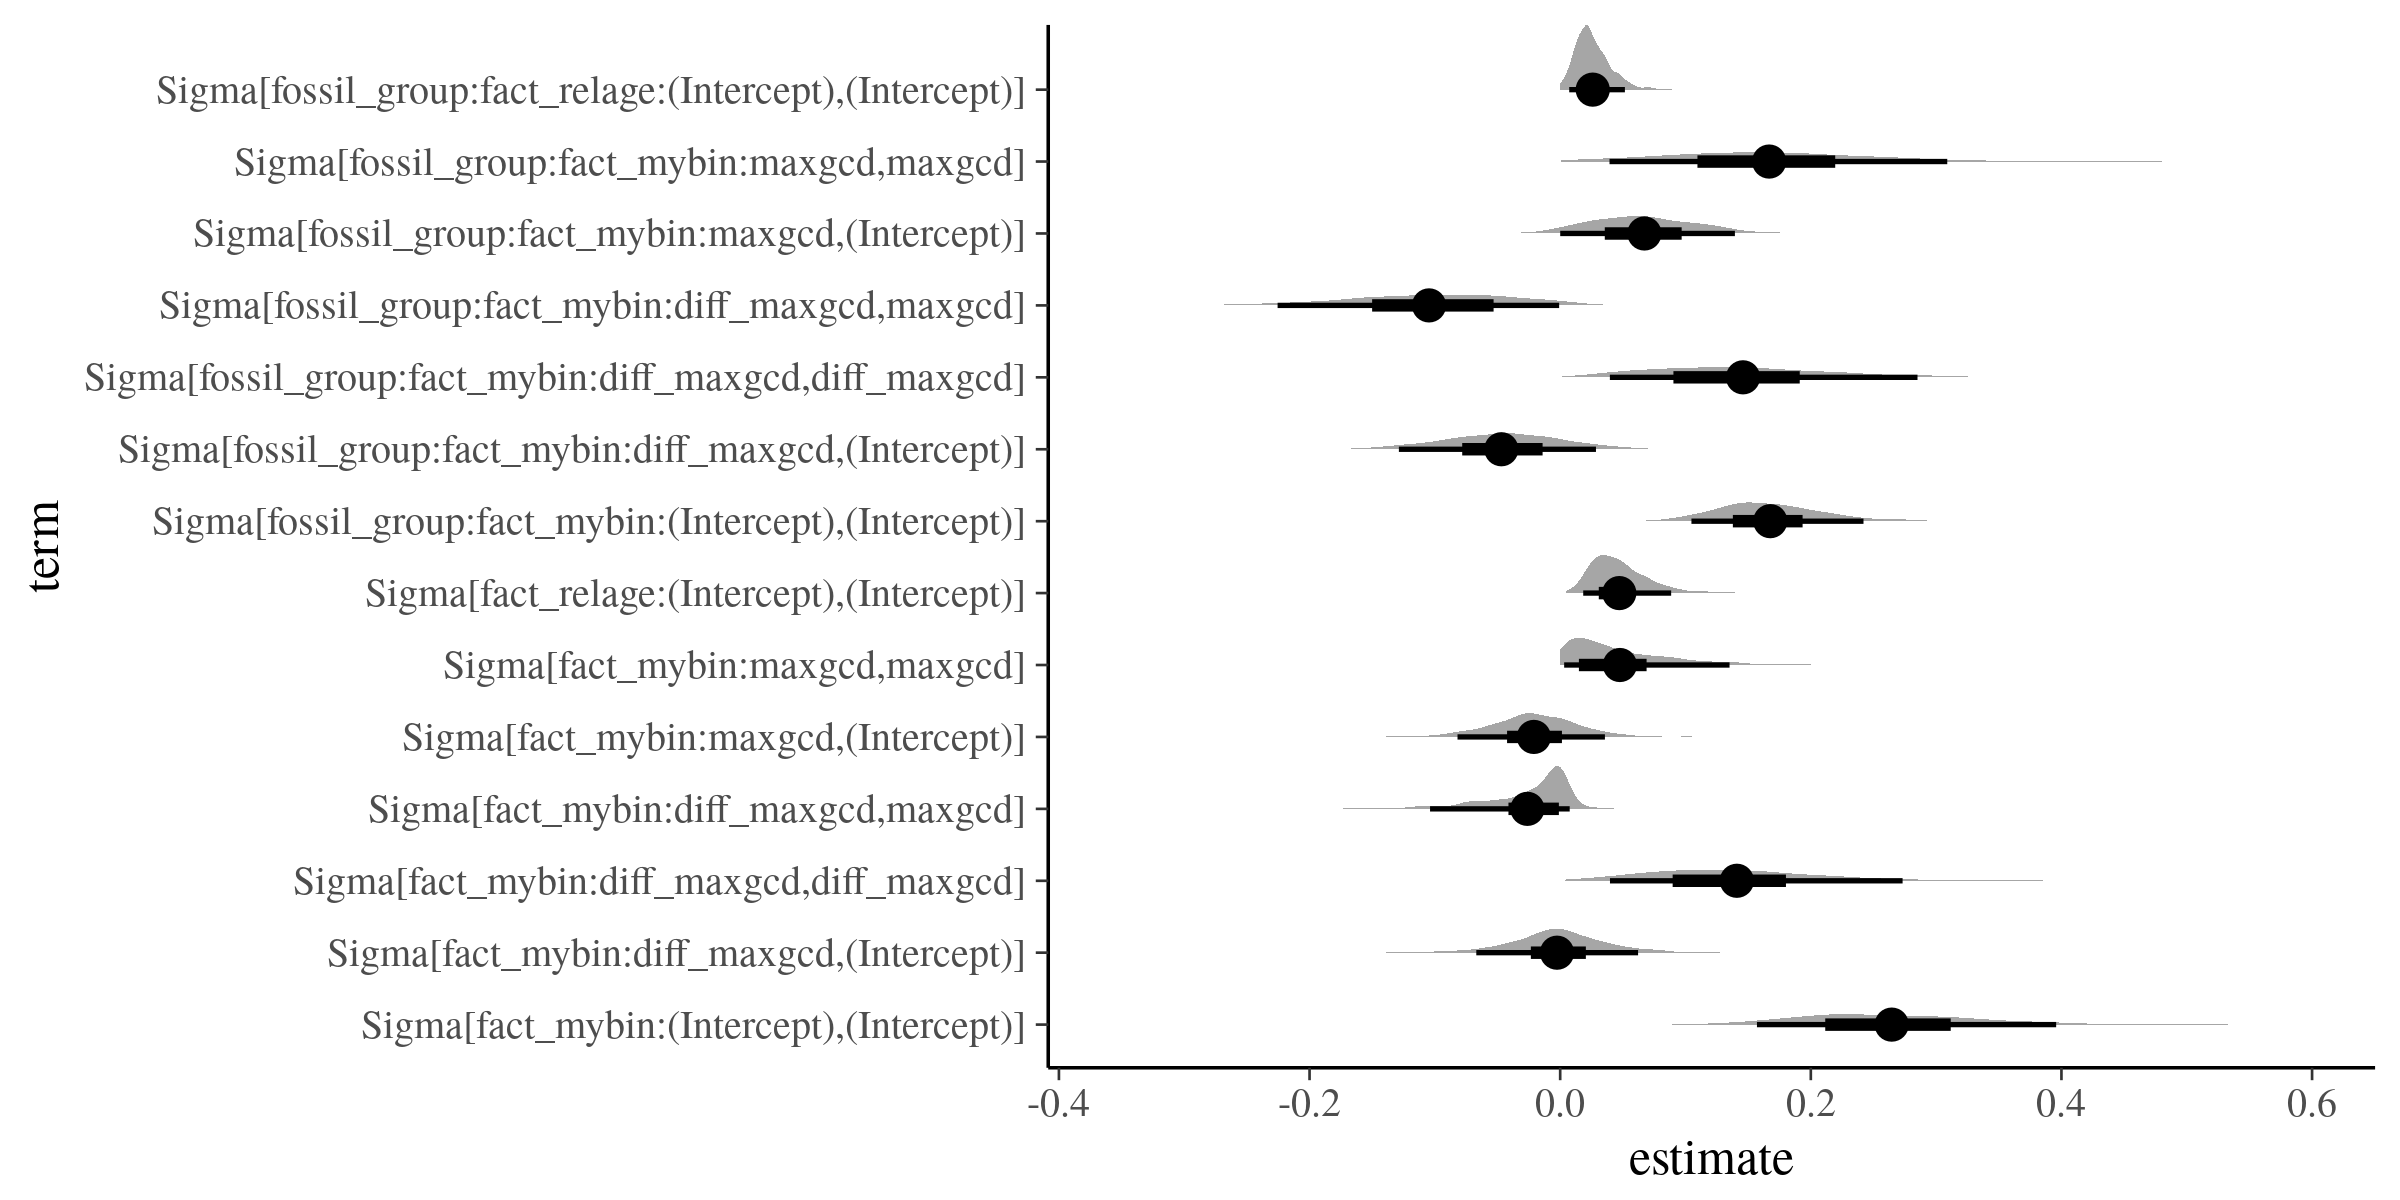
\includegraphics[width=\textwidth,height=0.5\textheight,keepaspectratio=true]{figure/variance_components}
  \caption{Contribution of multi-level components to unmodeled variance. Larger values indicate a greater contribution to overall variance. Variance components labeled as ``overall'' represent variance between grouping factors, while those labeled  ``within groups'' correspond to variance within grouping factors. If the overall component is greater than the within component, then the groupings do not structure the overall variance. If the within component is greater than the overall component, then the overall variance is structured by the groupings.}
  \label{fig:variance_components}
\end{figure}



Looking at four randomly sampled species, we evaluated their probability of extinction at all times that species was observed. We then compared these estimates to the geographic range trajectory of 


% risk estimate compared to change in geo-range
\begin{figure}[ht]
  \centering
  \begin{subfigure}{\textwidth}
    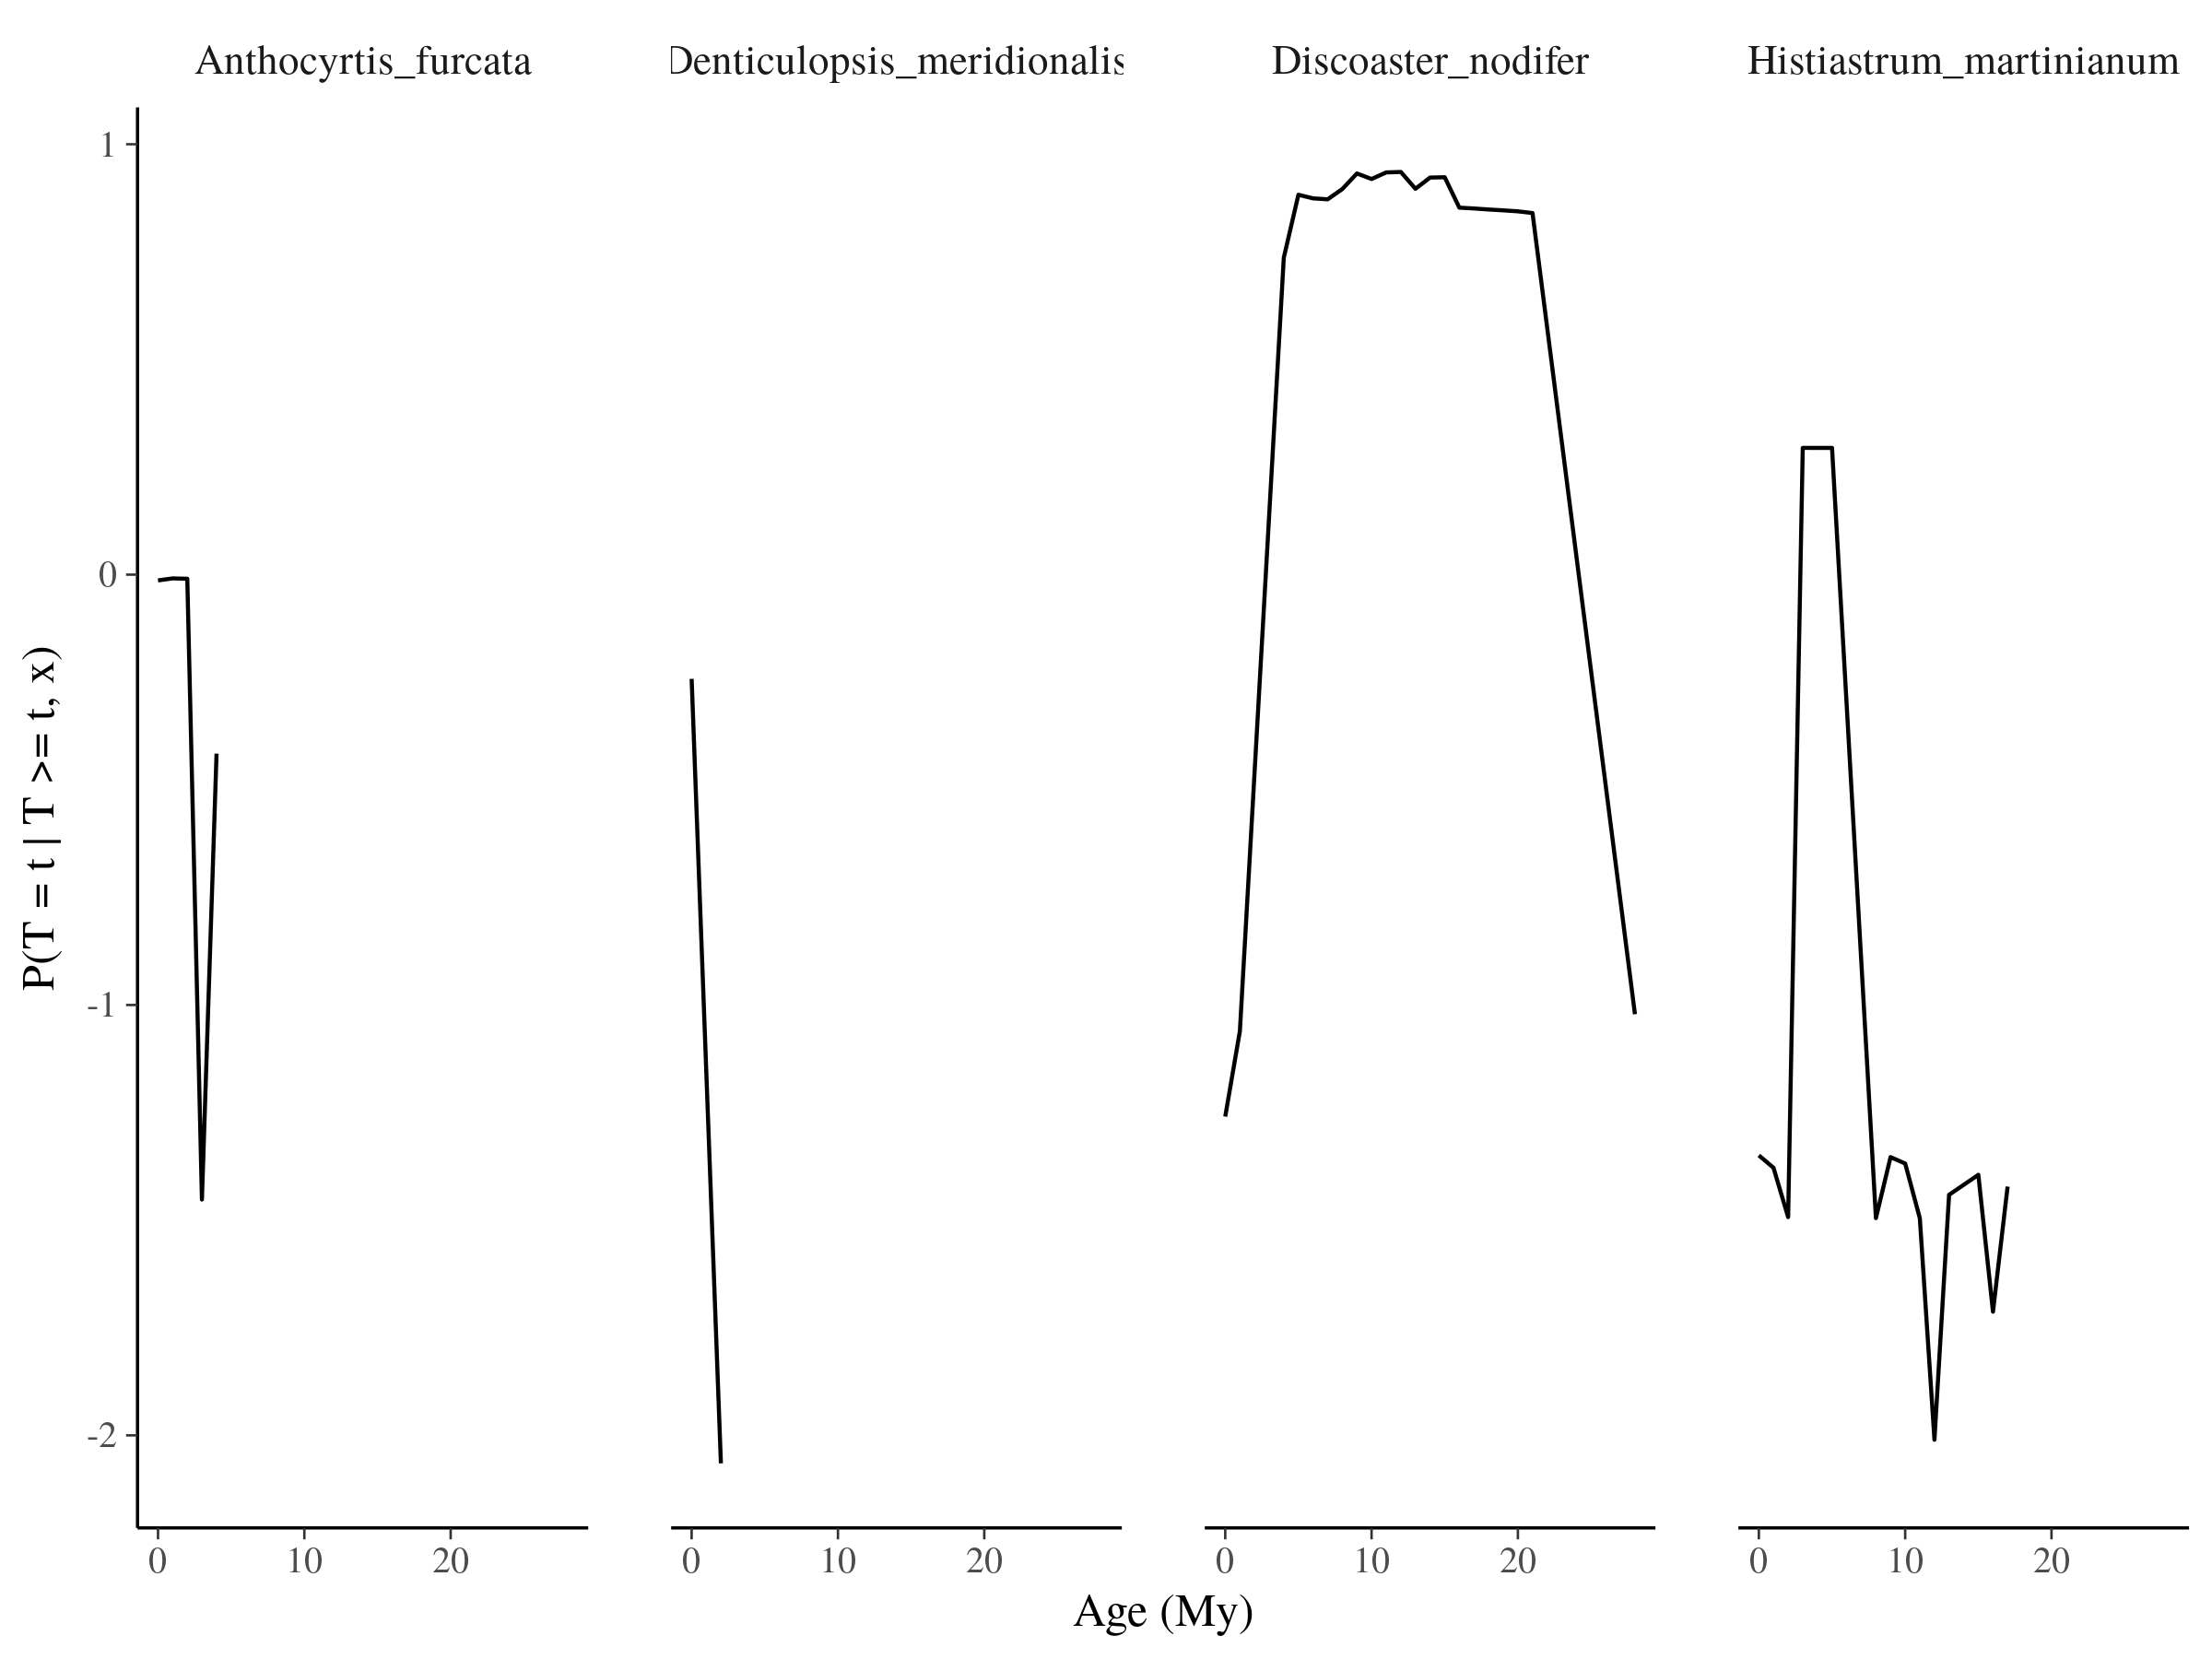
\includegraphics[width=\textwidth,height=0.5\textheight,keepaspectratio=true]{figure/relrisk_range}
    \caption{A}
    \label{fig:relrisk_range}
  \end{subfigure}

  \begin{subfigure}{\textwidth}
    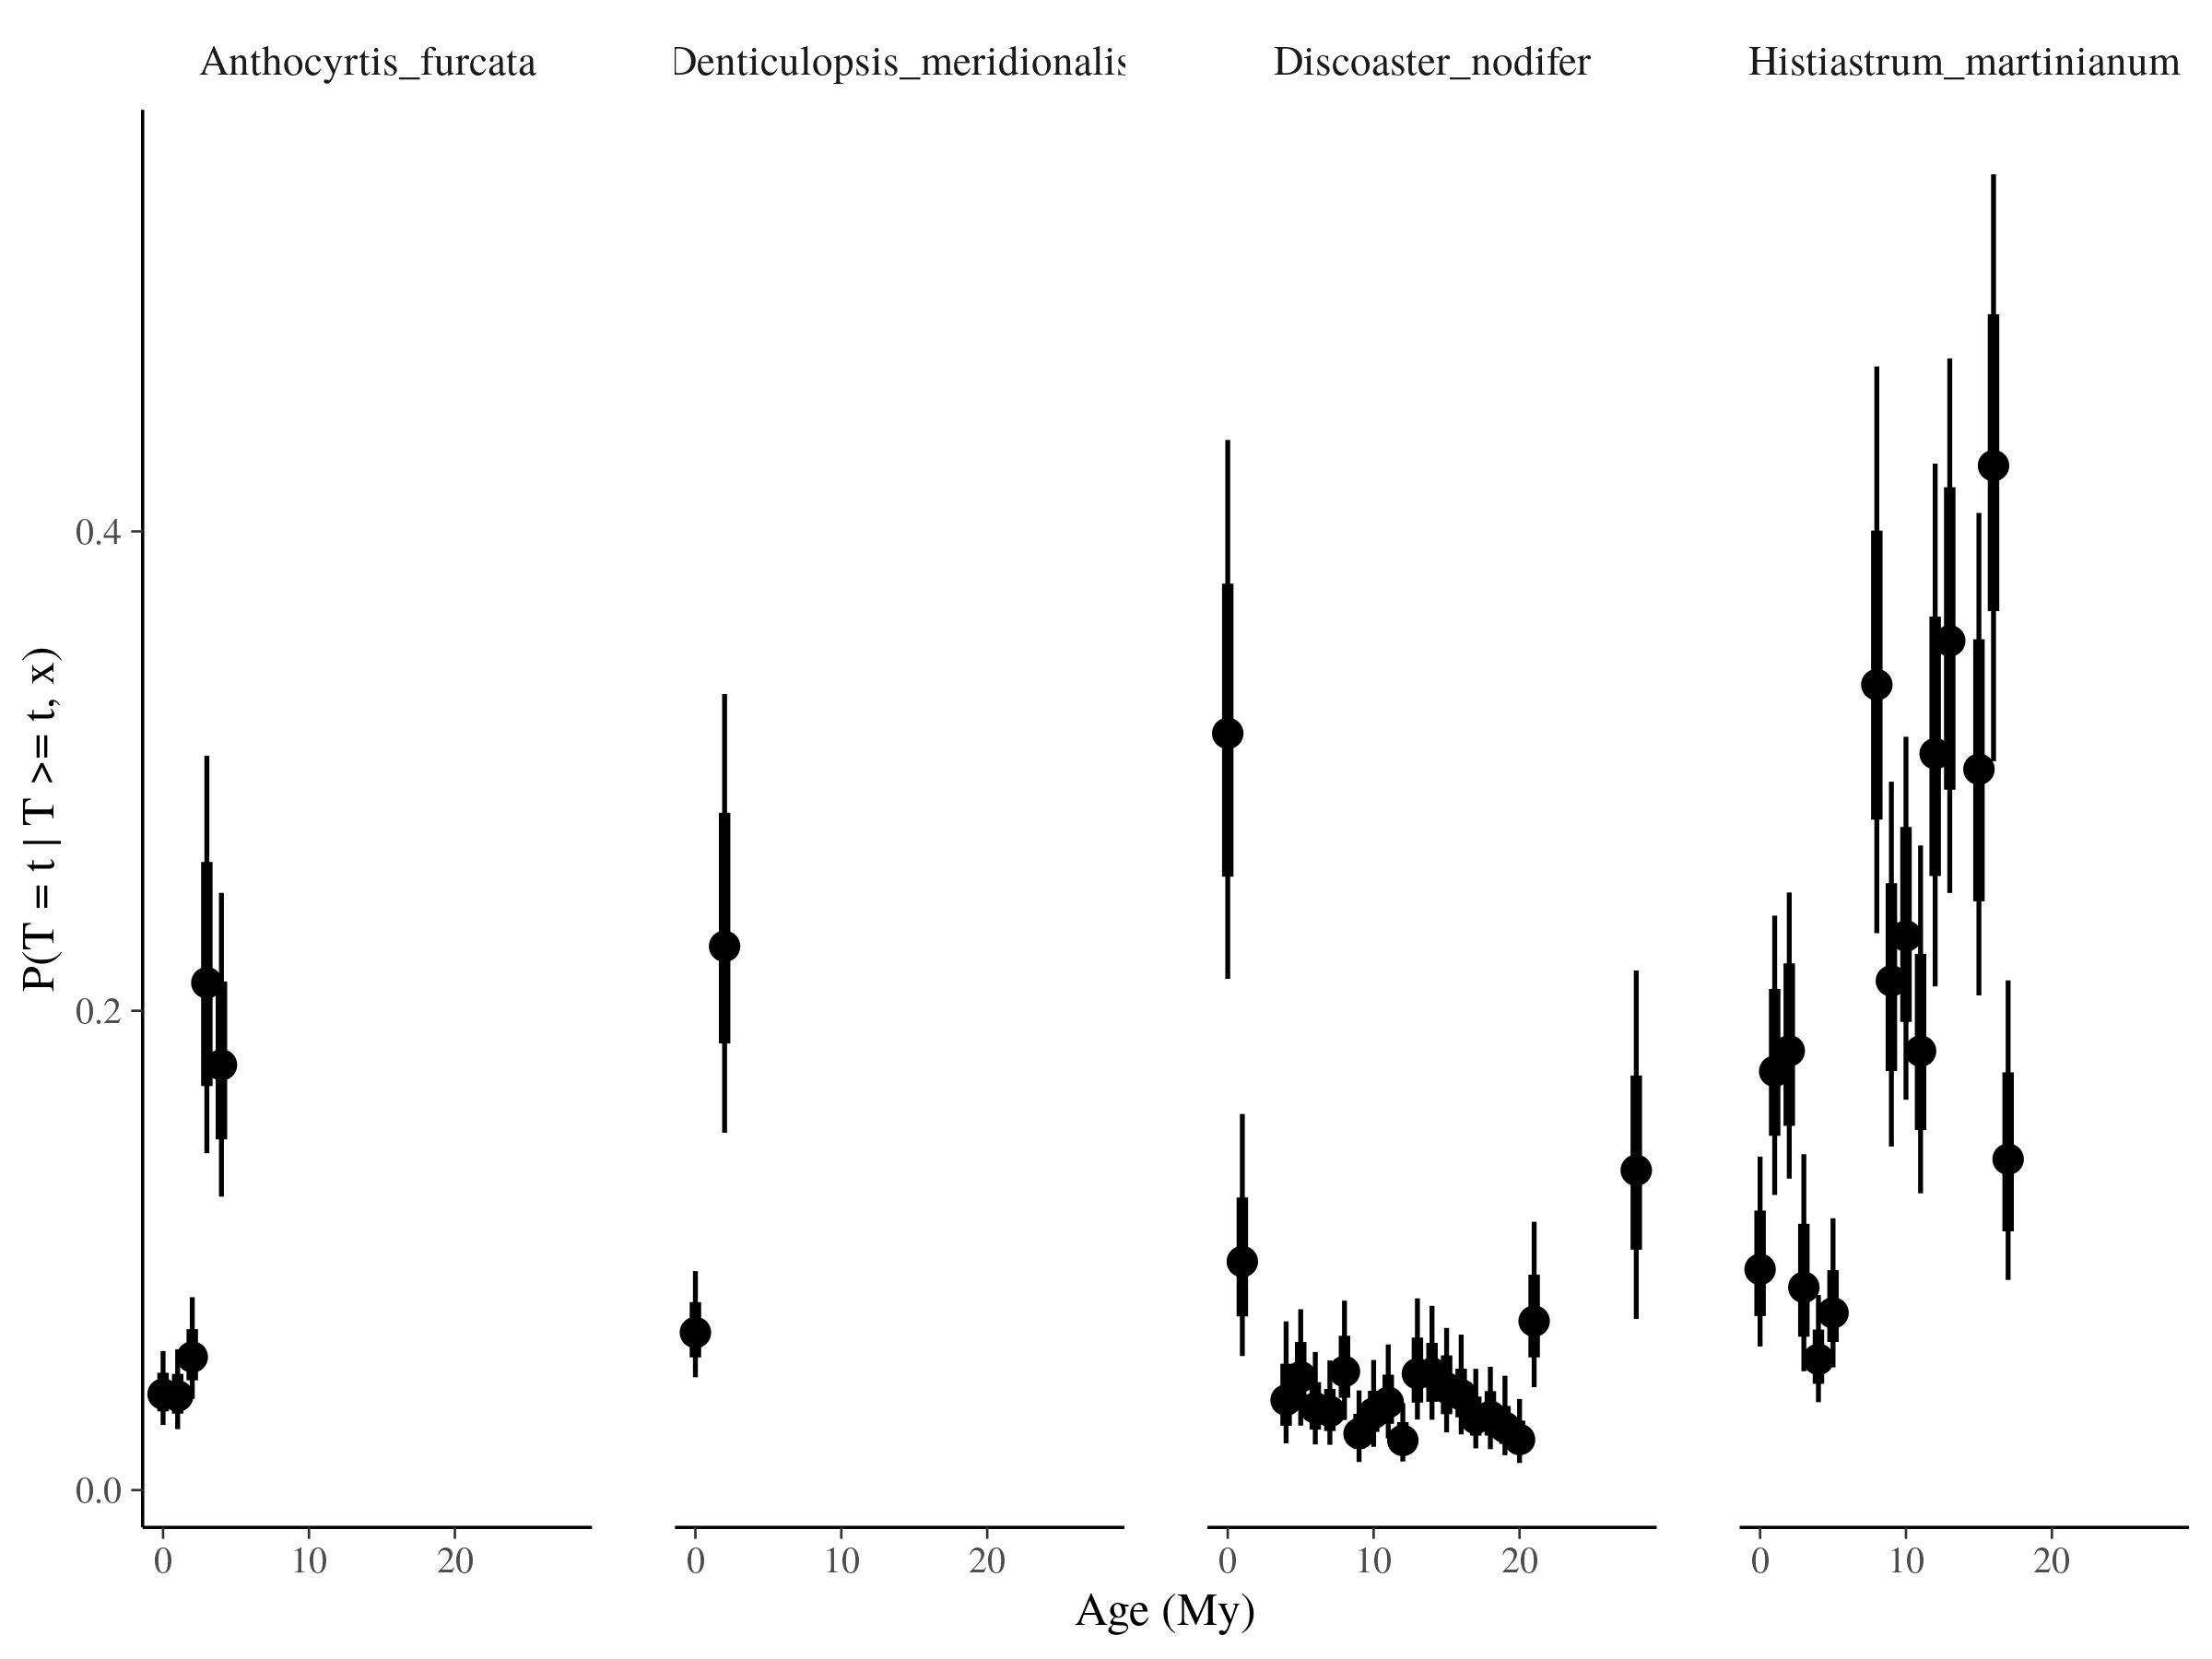
\includegraphics[width=\textwidth,height=0.5\textheight,keepaspectratio=true]{figure/relrisk_ext}
    \caption{B}
    \label{fig:relrisk_ext}
  \end{subfigure}
  \caption{Comparison between species geogrpahic range histories and our estimate of their probability of extinction for each time of observation. Geographic range is assumed observed without error. Our probability estimates are presented as a median (point) and 50\% and 80\% credible intervals.}
  \label{fig:relrisk_compare}
\end{figure}



\end{document}
